\documentclass[12pt,a4paper,oneside]{report}
\usepackage[utf8]{inputenc}
\usepackage[T1]{fontenc}
\usepackage[french]{babel}
\usepackage{graphicx}
\usepackage{lmodern}
\usepackage{geometry}
\usepackage{array}
\usepackage{setspace}
\usepackage[hidelinks]{hyperref}
\usepackage{enumitem}
\usepackage[svgnames,table]{xcolor}
\usepackage{textcomp}
\usepackage{booktabs}
\usepackage{tabularx}
\usepackage{longtable}
\usepackage{microtype}
\usepackage{float} % Résout les problèmes de texte qui dépasse des marges (Overfull \hbox)

% Configure enumitem
\setlist{nosep}
\setlist[itemize]{leftmargin=1.5em, topsep=0.2em, itemsep=0.15em}

% Robust Unicode mappings for copied text (French punctuation/spaces)
\DeclareUnicodeCharacter{00A0}{~}
\DeclareUnicodeCharacter{202F}{\,}
\DeclareUnicodeCharacter{2009}{\,}
\DeclareUnicodeCharacter{200B}{}
\DeclareUnicodeCharacter{00AD}{}
\DeclareUnicodeCharacter{20AC}{\texteuro}

\geometry{top=1.6cm,bottom=1.8cm,left=2.2cm,right=2.2cm}
\setstretch{1.15}
\setlength{\parindent}{1.2em}
\setlength{\parskip}{0pt}

% Correction de la macro logobox (ajout de \detokenize dans le fallback pour éviter l'erreur "Missing $")
% Placeholder pour les figures à insérer
\newcommand{\FIG}[1]{%
  \begin{center}
    \fbox{\parbox{0.85\textwidth}{\centering\small\textit{[Figure à insérer : #1]}}}
  \end{center}
}

\newcommand{\logobox}[2]{%
	\IfFileExists{\detokenize{#1}}{%
		\includegraphics[height=1.7cm]{\detokenize{#1}}%
	}{%
		\fbox{\parbox[c][2.0cm][c]{3.8cm}{\centering \small #2\\(ajoutez \detokenize{#1})}}%
	}%
}

\begin{document}
\hypersetup{pageanchor=false}
\begin{titlepage}
\begin{center}

\noindent
\begin{minipage}[c]{0.48\textwidth}
	\raggedright
	\IfFileExists{figures/Logo_INPT.png}{%
		
\includegraphics[height=1.6cm]{figures/Logo_INPT.png}%
	}{%
		\fbox{\parbox[c][1.6cm][c]{3.2cm}{\centering\small Logo INPT}}%
	}
\end{minipage}%
\begin{minipage}[c]{0.48\textwidth}
	\raggedleft
	\IfFileExists{figures/viseo-logo.png}{%
		
\includegraphics[width=3.8cm]{figures/viseo-logo.png}%
	}{%
		\fbox{\parbox[c][1.6cm][c]{3.8cm}{\centering\small Logo VISEO}}%
	}
\end{minipage}

\vspace{1.35cm}

{\fontsize{14}{16}\selectfont\textbf{M\'emoire du projet de fin d'\'etudes}}\\[0.45cm]
{\fontsize{11}{13}\selectfont POUR L'OBTENTION DU DIPL\^OME D'ING\'ENIEUR D'\'ETAT EN}\\[0.2cm]
{\fontsize{11}{13}\selectfont T\'EL\'ECOMMUNICATIONS ET TECHNOLOGIES DE L'INFORMATION}\\[0.4cm]
{\fontsize{16}{18}\selectfont \textbf{Fili\`ere : }\textit{INNOVATION ET AMOA}}

\vspace{0.35cm}
\rule{\textwidth}{0.6pt}

\vspace{0.65cm}

{\fontsize{21}{23}\selectfont\bfseries
Modernisation des processus d'achat :\\[0.2cm]
Impl\'ementation d'une solution Fiori RAP\\[0.2cm]
avec Agent IA conversationnel sous SAP BTP
}

\vspace{0.65cm}
\rule{\textwidth}{0.6pt}

\vspace{0.95cm}

\begin{flushleft}
\textit{R\'ealis\'e par :}\\[0.25cm]
{\fontsize{16}{18}\selectfont M. Anas ELWAHABI \& M. Mohamed Amine RAJAYI}
\end{flushleft}

\vspace{0.45cm}

\renewcommand{\arraystretch}{1.45}
\begin{tabular}{>{\raggedright\arraybackslash}p{0.48\textwidth} >{\centering\arraybackslash}p{0.13\textwidth} >{\raggedright\arraybackslash}p{0.28\textwidth}}
M. Abdellah ZAOUIA & INPT & - Encadrant \\
Mme. Sanna Mouzakki & VISEO & - Encadrante \\
\end{tabular}

\phantomsection
\vfill

\IfFileExists{figures/ZLAFA.png}{%
	
\includegraphics[width=0.48\textwidth]{figures/ZLAFA.png}
}{%
	\fbox{\parbox[c][2.2cm][c]{5.6cm}{\centering \small Embl\`eme INPT\\(ajoutez figures/ZLAFA.png)}}
}

\vspace{0.35cm}

{\small INSTITUT NATIONAL DES POSTES ET T\'EL\'ECOMMUNICATIONS}\\[0.25cm]
{\Large Ann\'ee universitaire : 2025/2026}

\end{center}
\end{titlepage}

\hypersetup{pageanchor=true}

% Pages liminaires
\pagenumbering{roman}
\setcounter{page}{1}

\chapter*{D\'edicace}
\phantomsection
\addcontentsline{toc}{chapter}{D\'edicace}
\label{sec:dedicace}
% A compl\'eter

\chapter*{Remerciements}
\phantomsection
\addcontentsline{toc}{chapter}{Remerciements}
\label{sec:remerciements}
% A compl\'eter

\chapter*{R\'esum\'e}
\phantomsection
\addcontentsline{toc}{chapter}{R\'esum\'e}
\label{sec:resume}
% A compl\'eter

\chapter*{Abstract}
\phantomsection
\addcontentsline{toc}{chapter}{Abstract}
\label{sec:abstract}
% To be completed

\chapter*{Nomenclature}
\phantomsection
\addcontentsline{toc}{chapter}{Nomenclature}
\label{sec:nomenclature}
{\normalsize
\renewcommand{\arraystretch}{0.82}
\begin{tabular}{p{0.18\textwidth}p{5\textwidth}}
ABAP        & Advanced Business Application Programming \\
ADT         & ABAP Development Tools \\
ALP         & Analytical List Page \\
API         & Application Programming Interface \\
BAPI        & Business Application Programming Interface \\
BCS         & Business Communication Services \\
BDEF        & Behavior Definition \\
BIL         & Behavior Implementation Layer \\
BO          & Business Object \\
BTP         & Business Technology Platform \\
CDS         & Core Data Services \\
CRUD        & Create, Read, Update, Delete \\
EKES        & Table SAP des confirmations de commandes \\
EKKO        & Table SAP des en-têtes de commandes d'achat \\
EKPO        & Table SAP des postes de commandes d'achat \\
EML         & Entity Manipulation Language \\
FLP         & Fiori Launchpad \\
HANA        & High-performance ANalytic Appliance \\
HTML        & HyperText Markup Language \\
HTTP        & HyperText Transfer Protocol \\
LIFNR       & Numéro fournisseur \\
LR          & List Report \\
ME22N/ME23N & Transactions de modification / affichage d'une commande d'achat \\
MM          & Materials Management \\
OData       & Open Data Protocol \\
PO          & Purchase Order \\
RAP         & RESTful Application Programming Model \\
S/4HANA     & SAP Business Suite 4 HANA \\
SAP         & Systeme, Anwendungen und Produkte in der Datenverarbeitung \\
SAP GUI     & SAP Graphical User Interface \\
SAPUI5      & SAP User Interface for HTML5 \\
SMTP        & Simple Mail Transfer Protocol \\
UI          & User Interface \\
UML         & Unified Modeling Language \\
USR21       & Table SAP utilisateur / numéro d'adresse \\
VDM         & Virtual Data Model \\
VS Code     & Visual Studio Code \\
\end{tabular}
}

\chapter*{Table des mati\`eres}
\phantomsection
\label{sec:toc-manuel}
\noindent\hyperref[sec:dedicace]{D\'edicace} \dotfill \pageref*{sec:dedicace}\\
\noindent\hyperref[sec:remerciements]{Remerciements} \dotfill \pageref*{sec:remerciements}\\
\noindent\hyperref[sec:resume]{R\'esum\'e} \dotfill \pageref*{sec:resume}\\
\noindent\hyperref[sec:abstract]{Abstract} \dotfill \pageref*{sec:abstract}\\
\noindent\hyperref[sec:nomenclature]{Nomenclature} \dotfill \pageref*{sec:nomenclature}\\
\noindent\hyperref[ch:intro-gen]{Introduction g\'en\'erale} \dotfill \pageref*{ch:intro-gen}\\
\noindent\hyperref[ch:contexte]{Chapitre 1 : Contexte g\'en\'eral du projet} \dotfill \pageref*{ch:contexte}\\
\noindent\hspace*{1em}\hyperref[ch1:introduction]{1.1 Introduction} \dotfill \pageref*{ch1:introduction}\\
\noindent\hspace*{1em}\hyperref[ch1:organisme]{1.2 Pr\'esentation de l'organisme d'accueil} \dotfill \pageref*{ch1:organisme}\\
\noindent\hspace*{2em}\hyperref[ch1:apercu]{1.2.1 Aper\c{c}u g\'en\'eral} \dotfill \pageref*{ch1:apercu}\\
\noindent\hspace*{2em}\hyperref[ch1:partenaires-viseo]{1.2.2 Partenaires du groupe VISEO} \dotfill \pageref*{ch1:partenaires-viseo}\\
\noindent\hspace*{2em}\hyperref[ch1:secteur]{1.2.3 Secteur d'activit\'e} \dotfill \pageref*{ch1:secteur}\\
\noindent\hspace*{2em}\hyperref[ch1:localisation]{1.2.4 Localisation et \'evolution} \dotfill \pageref*{ch1:localisation}\\
\noindent\hspace*{2em}\hyperref[ch1:domaines]{1.2.5 Domaines d'expertise} \dotfill \pageref*{ch1:domaines}\\
\noindent\hspace*{2em}\hyperref[ch1:chiffres]{1.2.6 Chiffres cl\'es} \dotfill \pageref*{ch1:chiffres}\\
\noindent\hspace*{2em}\hyperref[ch1:filiale]{1.2.7 Filiale Casablancaise : VI ONE NORTH AFRICA} \dotfill \pageref*{ch1:filiale}\\
\noindent\hspace*{3em}\hyperref[ch1:organigramme]{1.2.7.1 Organigramme} \dotfill \pageref*{ch1:organigramme}\\
\noindent\hspace*{1em}\hyperref[ch1:cahier]{1.3 Cahier des charges} \dotfill \pageref*{ch1:cahier}\\
\noindent\hspace*{2em}\hyperref[ch1:problematique]{1.3.1 Probl\'ematique} \dotfill \pageref*{ch1:problematique}\\
\noindent\hspace*{2em}\hyperref[ch1:objectifs]{1.3.2 Objectifs} \dotfill \pageref*{ch1:objectifs}\\
\noindent\hspace*{2em}\hyperref[ch1:perimetre]{1.3.3 P\'erim\`etre} \dotfill \pageref*{ch1:perimetre}\\
\noindent\hspace*{1em}\hyperref[ch1:gestion]{1.4 Gestion du projet} \dotfill \pageref*{ch1:gestion}\\
\noindent\hspace*{2em}\hyperref[ch1:methodologie]{1.4.1 M\'ethodologie adopt\'ee} \dotfill \pageref*{ch1:methodologie}\\
\noindent\hspace*{2em}\hyperref[ch1:planification]{1.4.2 Planification} \dotfill \pageref*{ch1:planification}\\
\noindent\hspace*{1em}\hyperref[ch1:conclusion]{1.5 Conclusion} \dotfill \pageref*{ch1:conclusion}\\
\noindent\hyperref[ch:existant]{Chapitre 2 : \'Etude et analyse de l'existant} \dotfill \pageref*{ch:existant}\\
\noindent\hspace*{1em}\hyperref[ch2:introduction]{2.1 Introduction} \dotfill \pageref*{ch2:introduction}\\
\noindent\hspace*{1em}\hyperref[ch2:erp]{2.2 Les syst\'emes ERP : concepts et r\'ole strat\'egique} \dotfill \pageref*{ch2:erp}\\
\noindent\hspace*{2em}\hyperref[ch2:erp-def]{2.2.1 D\'efinition et concepts fondamentaux} \dotfill \pageref*{ch2:erp-def}\\
\noindent\hspace*{2em}\hyperref[ch2:erp-role]{2.2.2 R\'ole strat\'egique et bénéfices} \dotfill \pageref*{ch2:erp-role}\\
\noindent\hspace*{2em}\hyperref[ch2:erp-evolution]{2.2.3 \'Evolution du mar\'ech\'e des ERP} \dotfill \pageref*{ch2:erp-evolution}\\
\noindent\hspace*{1em}\hyperref[ch2:sap]{2.3 Pr\'esentation de SAP : leader mondial} \dotfill \pageref*{ch2:sap}\\
\noindent\hspace*{2em}\hyperref[ch2:sap-historique]{2.3.1 Historique et position sur le march\'e} \dotfill \pageref*{ch2:sap-historique}\\
\noindent\hspace*{2em}\hyperref[ch2:sap-solutions]{2.3.2 Portefeuille de solutions SAP} \dotfill \pageref*{ch2:sap-solutions}\\
\noindent\hspace*{2em}\hyperref[ch2:sap-architecture]{2.3.3 Architecture modulaire et int\'egration SAP} \dotfill \pageref*{ch2:sap-architecture}\\
\noindent\hspace*{1em}\hyperref[ch2:mm]{2.4 Le module MM : cœur de la gestion des matériaux} \dotfill \pageref*{ch2:mm}\\
\noindent\hspace*{2em}\hyperref[ch2:mm-presentation]{2.4.1 Pr\'esentation g\'en\'erale du module MM} \dotfill \pageref*{ch2:mm-presentation}\\
\noindent\hspace*{2em}\hyperref[ch2:mm-role]{2.4.2 R\'ole critique dans les processus d'approvisionnement} \dotfill \pageref*{ch2:mm-role}\\
\noindent\hspace*{2em}\hyperref[ch2:mm-fonctionnalites]{2.4.3 Fonctionnalit\'es cl\'es du module MM} \dotfill \pageref*{ch2:mm-fonctionnalites}\\
\noindent\hspace*{3em}\hyperref[ch2:mm-approv]{2.4.3.1 Gestion des approvisionnements} \dotfill \pageref*{ch2:mm-approv}\\
\noindent\hspace*{3em}\hyperref[ch2:mm-stocks]{2.4.3.2 Gestion des stocks} \dotfill \pageref*{ch2:mm-stocks}\\
\noindent\hspace*{3em}\hyperref[ch2:mm-fourni]{2.4.3.3 Gestion des fournisseurs} \dotfill \pageref*{ch2:mm-fourni}\\
\noindent\hspace*{2em}\hyperref[ch2:mm-integration]{2.4.4 Int\'egration avec les autres modules SAP} \dotfill \pageref*{ch2:mm-integration}\\
\noindent\hspace*{3em}\hyperref[ch2:mm-int-sd]{2.4.4.1 Integration MM <-> SD (Ventes et Distribution)} \dotfill \pageref*{ch2:mm-int-sd}\\
\noindent\hspace*{3em}\hyperref[ch2:mm-int-pp]{2.4.4.2 Int\'egration MM <-> PP (Production)} \dotfill \pageref*{ch2:mm-int-pp}\\
\noindent\hspace*{3em}\hyperref[ch2:mm-int-fi]{2.4.4.3 Int\'egration MM <-> FI (Finance)} \dotfill \pageref*{ch2:mm-int-fi}\\
\noindent\hspace*{2em}\hyperref[ch2:mm-avantages]{2.4.5 Avantages strat\'egiques de SAP MM} \dotfill \pageref*{ch2:mm-avantages}\\
\noindent\hspace*{3em}\hyperref[ch2:mm-visibilite]{2.4.5.1 Am\'elioration de la visibilit\'e et du contr\'ole} \dotfill \pageref*{ch2:mm-visibilite}\\
\noindent\hspace*{3em}\hyperref[ch2:mm-optim]{2.4.5.2 Optimisation des processus et r\'eduction des coûts} \dotfill \pageref*{ch2:mm-optim}\\
\noindent\hspace*{3em}\hyperref[ch2:mm-decision]{2.4.5.3 Prise de d\'ecisions bas\'ee sur des donn\'ees} \dotfill \pageref*{ch2:mm-decision}\\
\noindent\hspace*{2em}\hyperref[ch2:mm-casusage]{2.4.6 Cas d'usage r\'eels et statistiques d'impl\'ementation} \dotfill \pageref*{ch2:mm-casusage}\\
\noindent\hspace*{2em}\hyperref[ch2:mm-organisation]{2.4.7 Structure organisationnelle et entit\'es du module MM} \dotfill \pageref*{ch2:mm-organisation}\\
\noindent\hspace*{3em}\hyperref[ch2:mm-org-niveaux]{2.4.7.1 Niveaux hi\'erarchiques organisationnels} \dotfill \pageref*{ch2:mm-org-niveaux}\\
\noindent\hspace*{2em}\hyperref[ch2:mm-transactions]{2.4.8 Transactions SAP et codes de transaction (T-codes)} \dotfill \pageref*{ch2:mm-transactions}\\
\noindent\hspace*{2em}\hyperref[ch2:mm-approv-process]{2.4.9 Processus d'approvisionnement : taxonomie et strat\'egies} \dotfill \pageref*{ch2:mm-approv-process}\\
\noindent\hspace*{3em}\hyperref[ch2:mm-approv-base]{2.4.9.1 Approvisionnement de base (Standard Procurement)} \dotfill \pageref*{ch2:mm-approv-base}\\
\noindent\hspace*{3em}\hyperref[ch2:mm-approv-special]{2.4.9.2 Approvisionnement sp\'ecialis\'e (Special Procurement)} \dotfill \pageref*{ch2:mm-approv-special}\\
\noindent\hspace*{2em}\hyperref[ch2:mm-flux-transactionnel]{2.4.10 Flux transactionnel complet du module MM} \dotfill \pageref*{ch2:mm-flux-transactionnel}\\
\noindent\hspace*{3em}\hyperref[ch2:mm-flux-demandes]{2.4.10.1 Processus de cr\'eation et gestion des demandes} \dotfill \pageref*{ch2:mm-flux-demandes}\\
\noindent\hspace*{3em}\hyperref[ch2:mm-flux-commande]{2.4.10.2 Processus de commande d'achat (Purchase Order)} \dotfill \pageref*{ch2:mm-flux-commande}\\
\noindent\hspace*{3em}\hyperref[ch2:mm-flux-reception]{2.4.10.3 Processus de r\'eception et facturation} \dotfill \pageref*{ch2:mm-flux-reception}\\
\noindent\hspace*{2em}\hyperref[ch2:mm-purchase-order]{2.4.11 Structure et informations des commandes d'achat} \dotfill \pageref*{ch2:mm-purchase-order}\\
\noindent\hspace*{3em}\hyperref[ch2:mm-po-entete]{2.4.11.1 Donn\'ees d'en-t\^ete de la commande} \dotfill \pageref*{ch2:mm-po-entete}\\
\noindent\hspace*{3em}\hyperref[ch2:mm-po-lignes]{2.4.11.2 Donn\'ees de lignes de la commande} \dotfill \pageref*{ch2:mm-po-lignes}\\
\noindent\hspace*{2em}\hyperref[ch2:mm-arch-tech]{2.4.12 Architecture technique de SAP} \dotfill \pageref*{ch2:mm-arch-tech}\\
\noindent\hspace*{3em}\hyperref[ch2:mm-arch-pres]{2.4.12.1 Couche de pr\'esentation} \dotfill \pageref*{ch2:mm-arch-pres}\\
\noindent\hspace*{3em}\hyperref[ch2:mm-arch-app]{2.4.12.2 Couche applicative} \dotfill \pageref*{ch2:mm-arch-app}\\
\noindent\hspace*{3em}\hyperref[ch2:mm-arch-bdd]{2.4.12.3 Couche base de donn\'ees} \dotfill \pageref*{ch2:mm-arch-bdd}\\
\noindent\hspace*{2em}\hyperref[ch2:mm-paysage-systeme]{2.4.13 Organisation et paysage du syst\`eme SAP} \dotfill \pageref*{ch2:mm-paysage-systeme}\\
\noindent\hspace*{3em}\hyperref[ch2:mm-landscape]{2.4.13.1 Paysage syst\`eme (System Landscape)} \dotfill \pageref*{ch2:mm-landscape}\\
\noindent\hspace*{3em}\hyperref[ch2:mm-transport-orders]{2.4.13.2 Ordres de transport (Transport Orders - OT)} \dotfill \pageref*{ch2:mm-transport-orders}\\
\noindent\hspace*{1em}\hyperref[ch2:tech]{2.5 Technologies SAP utilis\'ees} \dotfill \pageref*{ch2:tech}\\
\noindent\hspace*{2em}\hyperref[ch2:odata]{2.5.1 OData} \dotfill \pageref*{ch2:odata}\\
\noindent\hspace*{2em}\hyperref[ch2:rap]{2.5.2 RAP} \dotfill \pageref*{ch2:rap}\\
\noindent\hspace*{2em}\hyperref[ch2:sapui5]{2.5.3 SAPUI5} \dotfill \pageref*{ch2:sapui5}\\
\noindent\hspace*{1em}\hyperref[ch2:conclusion]{2.6 Conclusion} \dotfill \pageref*{ch2:conclusion}\\
\noindent\hyperref[ch:analyse-conception]{Chapitre 3 : Analyse et conception de la solution} \dotfill \pageref*{ch:analyse-conception}\\
\noindent\hspace*{1em}\hyperref[ch3:introduction]{3.1 Introduction} \dotfill \pageref*{ch3:introduction}\\
\noindent\hspace*{1em}\hyperref[ch3:demarche]{3.2 Démarche méthodologique et répartition des tâches} \dotfill \pageref*{ch3:demarche}\\
\noindent\hspace*{1em}\hyperref[ch3:analyse-besoins]{3.3 Ingénierie des exigences et spécifications} \dotfill \pageref*{ch3:analyse-besoins}\\
\noindent\hspace*{2em}\hyperref[ch3:besoins-f]{3.3.1 Exigences fonctionnelles métiers} \dotfill \pageref*{ch3:besoins-f}\\
\noindent\hspace*{2em}\hyperref[ch3:besoins-nf]{3.3.2 Exigences non fonctionnelles et architecturales} \dotfill \pageref*{ch3:besoins-nf}\\
\noindent\hspace*{1em}\hyperref[ch3:cas-util]{3.4 Modélisation des processus et Cas d'utilisation} \dotfill \pageref*{ch3:cas-util}\\
\noindent\hspace*{1em}\hyperref[ch3:architecture]{3.5 Architecture globale et choix technologiques} \dotfill \pageref*{ch3:architecture}\\
\noindent\hspace*{1em}\hyperref[ch3:uml]{3.6 Conception détaillée et modélisation} \dotfill \pageref*{ch3:uml}\\
\noindent\hspace*{2em}\hyperref[ch3:diag-classes]{3.6.1 Modèle de données} \dotfill \pageref*{ch3:diag-classes}\\
\noindent\hspace*{2em}\hyperref[ch3:diag-sequences]{3.6.2 Flux transactionnels et asynchronisme} \dotfill \pageref*{ch3:diag-sequences}\\
\noindent\hspace*{1em}\hyperref[ch3:ia-joule]{3.7 Stratégie d'automatisation et Agent IA (SAP Joule)} \dotfill \pageref*{ch3:ia-joule}\\
\noindent\hspace*{1em}\hyperref[ch3:conclusion]{3.8 Conclusion} \dotfill \pageref*{ch3:conclusion}\\
\noindent\hyperref[ch:archi-tech]{Chapitre 4 : Conception d\'etaill\'ee et architecture technique} \dotfill \pageref*{ch:archi-tech}\\
\noindent\hspace*{1em}\hyperref[ch4:introduction]{4.1 Introduction} \dotfill \pageref*{ch4:introduction}\\
\noindent\hspace*{1em}\hyperref[ch4:architecture]{4.2 Architecture globale de la solution} \dotfill \pageref*{ch4:architecture}\\
\noindent\hspace*{1em}\hyperref[ch4:cds]{4.3 Mod\'elisation CDS} \dotfill \pageref*{ch4:cds}\\
\noindent\hspace*{1em}\hyperref[ch4:odata-logique]{4.4 Services OData et logique m\'etier} \dotfill \pageref*{ch4:odata-logique}\\
\noindent\hspace*{1em}\hyperref[ch4:conclusion]{4.5 Conclusion} \dotfill \pageref*{ch4:conclusion}\\
\noindent\hyperref[ch:dev-real]{Chapitre 5 : D\'eveloppement et r\'ealisation} \dotfill \pageref*{ch:dev-real}\\
\noindent\hspace*{1em}\hyperref[ch5:introduction]{5.1 Introduction} \dotfill \pageref*{ch5:introduction}\\
\noindent\hspace*{1em}\hyperref[ch5:env]{5.2 Environnement de d\'eveloppement} \dotfill \pageref*{ch5:env}\\
\noindent\hspace*{1em}\hyperref[ch5:implementation]{5.3 Impl\'ementation} \dotfill \pageref*{ch5:implementation}\\
\noindent\hspace*{2em}\hyperref[ch5:auth]{5.3.1 Authentification} \dotfill \pageref*{ch5:auth}\\
\noindent\hspace*{2em}\hyperref[ch5:consult]{5.3.2 Application de consultation} \dotfill \pageref*{ch5:consult}\\
\noindent\hspace*{2em}\hyperref[ch5:conf-rejet]{5.3.3 Application de confirmation/rejet} \dotfill \pageref*{ch5:conf-rejet}\\
\noindent\hspace*{2em}\hyperref[ch5:masse]{5.3.4 Confirmation en masse} \dotfill \pageref*{ch5:masse}\\
\noindent\hspace*{1em}\hyperref[ch5:reporting]{5.4 Volet reporting} \dotfill \pageref*{ch5:reporting}\\
\noindent\hspace*{2em}\hyperref[ch5:etl]{5.4.1 Cha\^ine ETL et entrep\^ot de donn\'ees} \dotfill \pageref*{ch5:etl}\\
\noindent\hspace*{2em}\hyperref[ch5:pbi]{5.4.2 Tableaux de bord Power BI} \dotfill \pageref*{ch5:pbi}\\
\noindent\hspace*{1em}\hyperref[ch5:joule]{5.5 Agent conversationnel Joule} \dotfill \pageref*{ch5:joule}\\
\noindent\hspace*{2em}\hyperref[ch5:joule-archi]{5.5.1 Architecture de bout en bout} \dotfill \pageref*{ch5:joule-archi}\\
\noindent\hspace*{2em}\hyperref[ch5:joule-dest]{5.5.2 Configuration Cloud Connector et Destination BTP} \dotfill \pageref*{ch5:joule-dest}\\
\noindent\hspace*{2em}\hyperref[ch5:joule-skills]{5.5.3 Conception des skills Joule} \dotfill \pageref*{ch5:joule-skills}\\
\noindent\hspace*{2em}\hyperref[ch5:joule-agent]{5.5.4 Orchestration via SupplierPortalAssistant} \dotfill \pageref*{ch5:joule-agent}\\
\noindent\hspace*{2em}\hyperref[ch5:joule-demo]{5.5.5 Exemples de conversations} \dotfill \pageref*{ch5:joule-demo}\\
\noindent\hspace*{1em}\hyperref[ch5:tests]{5.6 Tests et validation} \dotfill \pageref*{ch5:tests}\\
\noindent\hspace*{1em}\hyperref[ch5:conclusion]{5.7 Conclusion} \dotfill \pageref*{ch5:conclusion}\\
\noindent\hyperref[ch:conclusion]{Conclusion g\'en\'erale et perspectives} \dotfill \pageref*{ch:conclusion}\\
\noindent\hyperref[ch:references]{R\'ef\'erences} \dotfill \pageref*{ch:references}

\listoffigures
\listoftables

% Corps du rapport
\clearpage
\pagenumbering{arabic}
\setcounter{page}{1}

\chapter*{Introduction g\'en\'erale}
\phantomsection
\addcontentsline{toc}{chapter}{Introduction g\'en\'erale}
\label{ch:intro-gen}
\begingroup
\setlength{\parindent}{1.2em}
\setlength{\parskip}{0pt}

Dans un contexte de digitalisation croissante des échanges, l'optimisation de la relation
fournisseur constitue un enjeu stratégique majeur pour les entreprises. Au sein des
environnements \textbf{SAP S/4HANA}, le processus de confirmation des commandes d'achat
souffre de plusieurs lacunes : saisie manuelle par les acheteurs, absence de traçabilité
des rejets et aucun accès autonome pour les fournisseurs. C'est dans ce cadre que s'inscrit
ce projet de fin d'études, réalisé au sein de \textit{VI-ONE North Africa (groupe VISEO)},
en partenariat avec l'\textbf{INPT} de Rabat.

L'objectif est de concevoir un \textbf{Portail Fournisseur} sur SAP S/4HANA, fondé sur
le framework \textbf{RAP} et les services \textbf{OData V4}, permettant aux fournisseurs
de consulter leurs commandes, de les confirmer (unitairement ou en masse), de rejeter des
postes avec motif traçable et de recevoir des notifications automatiques par email.
Ce portail est enrichi d'un \textbf{agent conversationnel Joule} déployé sur \textbf{SAP BTP},
qui permet aux utilisateurs d'interagir avec l'ensemble de ces fonctionnalités en langage
naturel --- consulter, confirmer ou rejeter des commandes par simple message, sans naviguer
dans les écrans Fiori.

Ce rapport est structuré en cinq chapitres :

\begin{itemize}[label=---,itemsep=0.15em,topsep=0.2em]
\item \textbf{Chapitre 1 : Présentation de l'organisme d'accueil} ---
Présentation de VISEO, VI-ONE North Africa, de l'INPT, du cadre du PFE,
de la problématique et de la conduite du projet.
\item \textbf{Chapitre 2 : État de l'art} ---
Systèmes ERP, plateforme SAP et module MM, technologies mobilisées
(RAP, CDS Views, OData V4, SAPUI5, SAP BTP et Joule).
\item \textbf{Chapitre 3 : Étude et analyse de l'existant} ---
Limites du processus actuel, analyse des solutions existantes
et justification des choix technologiques.
\item \textbf{Chapitre 4 : Analyse et conception} ---
Besoins fonctionnels et non fonctionnels, modélisation UML,
architecture en couches, maquettes et sécurité des données.
\item \textbf{Chapitre 5 : Développement et réalisation} ---
Backend RAP, frontend Fiori Elements, intégration au Fiori Launchpad
et agent conversationnel Joule (skills, orchestration, exemples de conversations).
\end{itemize}


\endgroup
\chapter{Présentation de l’organisme d’accueil}\label{ch:contexte}
\section{Introduction}\label{ch1:introduction}

Ce premier chapitre vise \`a pr\'esenter de mani\`ere exhaustive le contexte g\'en\'eral
dans lequel le projet s'est d\'eroul\'e. Nous d\'ebuterons par une pr\'esentation descriptive
du groupe VISEO, mettant en lumi\`ere ses missions, ses r\'ef\'erences et sa structure
organisationnelle. Ensuite, nous pr\'esenterons l'environnement de travail, \`a savoir
l'ERP SAP et ses diff\'erents modules, en nous focalisant sur le module MM. Nous aborderons
\'egalement le cahier des charges qui d\'efinit les contours et les attentes du projet.
Enfin, nous discuterons du pilotage du projet, en pr\'esentant les m\'ethodologies de gestion
retenues pour mener \`a bien ce travail.

\vspace{0.3cm}

Le projet s'inscrit dans le cadre des activit\'es de l'\textbf{\'equipe technique SAP S/4}
au sein de Vi-One North Africa. \`A la suite d'une \textbf{formation intensive de deux mois}
portant sur l'ERP SAP --- couvrant aussi bien les fondamentaux fonctionnels que les aspects
techniques de la plateforme --- nous avons \'et\'e affect\'es \`a cette \'equipe sp\'ecialis\'ee,
ce qui a constitu\'e une immersion concr\`ete et structurante dans l'\'ecosyst\`eme SAP
en environnement professionnel.

\vspace{0.2cm}

L'\'equipe SAP S/4 est compos\'ee de deux profils de consultants aux r\^oles compl\'ementaires :

\begin{itemize}[label=\textbullet, itemsep=0.2em]
  \item \textbf{Consultants SAP techniques} : ils prennent en charge les d\'eveloppements
        sp\'ecifiques, l'int\'egration de nouvelles fonctionnalit\'es et la personnalisation
        de la plateforme SAP en fonction des besoins m\'etier de chaque client. Leur expertise
        couvre notamment les langages ABAP, les services OData et le framework RAP.
  \item \textbf{Consultants SAP fonctionnels} : ils assurent la conception des solutions,
        la r\'ealisation des tests fonctionnels et le suivi de ces derniers afin de garantir
        la conformit\'e des livrables aux sp\'ecifications d\'efinies. Ils constituent
        l'interface privil\'egi\'ee entre les \'equipes m\'etier des clients et les
        d\'eveloppeurs techniques.
\end{itemize}

\vspace{0.1cm}

C'est dans ce cadre collaboratif et exigeant que s'est inscrit notre projet de fin d'\'etudes,
alliant comp\'etences fonctionnelles et techniques pour concevoir et d\'evelopper un
\textbf{Portail Fournisseur} sur la plateforme SAP.
\section{Pr\'esentation de l'organisme d'accueil}\label{ch1:organisme}
\subsection{Aper\c{c}u g\'en\'eral}\label{ch1:apercu}
\vspace{0.3cm}

\begin{figure}[htbp]
\centering
\IfFileExists{figures/viseo-logo.png}{%
	
\includegraphics[width=0.35\textwidth]{figures/viseo-logo.png}
}{%
	\fbox{\parbox[c][1.75cm][c]{4cm}{\centering \small Logo VISEO\\(ajoutez figures/viseo-logo.png)}}%
}
\caption{Logo du groupe VISEO}
\end{figure}
Le groupe VISEO, fond\'e en 1999 par Olivier DHIONTE, actuel PDG de l'entreprise, est une
entreprise fran\c{c}aise de services du num\'erique (ESN) \'etablie \`a Boulogne-Billancourt. Depuis ses
d\'ebuts, VISEO s'est impos\'e comme un leader dans le secteur du conseil et de l'int\'egration
informatique, offrant des solutions innovantes et des services spcialis\'es pour transformer les
processus m\'etier des grandes entreprises.

Avec une forte expertise dans les domaines de l'ERP (notamment SAP), de la mobilit\'e, du
cloud computing et de l'intelligence artificielle, VISEO accompagne ses clients dans la modernisation
de leurs syst\`emes d'information et l'optimisation de leurs op\'erations. Fort d'une \'equipe de plus
de 500 collaborateurs distribu\'es dans plusieurs pays, le groupe VISEO maintient une pr\'esence
strat\'egique en Europe, en Afrique et au-del\`a, en proposant des services de haute qualit\'e
adapt\'es aux besoins sp\'ecifiques de chaque march\'e.
\vspace{0.4cm}

\begin{table}[htbp]
\centering
\renewcommand{\arraystretch}{1.75}
\setlength{\tabcolsep}{14pt}
\renewcommand{\tabularxcolumn}[1]{m{#1}}
\rowcolors{3}{RoyalBlue!7}{white}
\begin{tabularx}{\textwidth}{>{\bfseries\color{MidnightBlue}\raggedright\arraybackslash}m{5.2cm} >{\raggedright\arraybackslash}X}
\toprule
\rowcolor{RoyalBlue!65}
\textcolor{white}{\textbf{\large Fiche d'identité}} & \textcolor{white}{\textbf{\large Groupe VISEO}} \\
\midrule
NOM & « VISEO » \\
FORME JURIDIQUE & Société Anonyme \\
DATE DE CRÉATION & 1999 \\
SECTEUR D'ACTIVITÉ & Systèmes d'information, ERP, Digital, Technologies, Process et Data \\
CHIFFRE D'AFFAIRES & 265 M Euros \\
CAPITAL & 4 579 015 € \\
SIÈGE SOCIAL & 105, rue Marcel Dassault, 92100 Boulogne-Billancourt, France \\
TÉLÉPHONE & +33 1 71 19 46 30 \\
EFFECTIFS & 2500 collaborateurs \\
LOCALISATION & France, Allemagne, États-Unis, Maroc, Chine, Singapour, Australie \\
\bottomrule
\end{tabularx}
\caption{Fiche d'identité du groupe VISEO}
\end{table}

\vspace{0.5cm}



\subsection{Partenaires du groupe VISEO}\label{ch1:partenaires-viseo}

Le groupe VISEO s'appuie sur un r\'eseau solide de partenariats strat\'egiques avec les
leaders mondiaux des technologies de l'information. Ces alliances lui permettent de
proposer des solutions compl\`etes et innovantes, en combinant son expertise m\'etier avec
les technologies les plus avanc\'ees du march\'e. Qu'il s'agisse de solutions ERP, de
plateformes cloud ou d'outils analytiques, chaque partenariat renforce la capacit\'e de
VISEO \`a r\'epondre aux besoins sp\'ecifiques de ses clients avec un niveau d'excellence
reconnu \`a l'\'echelle internationale. Les figures ci-dessous illustrent l'\'ecosyst\`eme
partenarial de VISEO, refl\'etant la diversit\'e et la compl\'ementarit\'e des collaborations
\'etablies sur l'ensemble de ses domaines d'activit\'e.

\begin{figure}[h!]
\centering
\begin{minipage}[t]{0.48\textwidth}
\centering
\IfFileExists{figures/partenaire viseo.jpg}{%
  
\includegraphics[width=\textwidth]{figures/partenaire viseo.jpg}
}{%
  \fbox{\parbox[c][3.5cm][c]{\linewidth}{\centering \small Partenaires VISEO\\(ajoutez figures/partenaire viseo.jpg)}}%
}

\vspace{0.2cm}
{\small\textit{(a) Partenaires du groupe VISEO -- partie 1}}
\end{minipage}
\hfill
\begin{minipage}[t]{0.48\textwidth}
\centering
\IfFileExists{figures/partenaire viseo 1.jpg}{%
  
\includegraphics[width=\textwidth]{figures/partenaire viseo 1.jpg}
}{%
  \fbox{\parbox[c][3.5cm][c]{\linewidth}{\centering \small Partenaires VISEO\\(ajoutez figures/partenaire viseo 1.jpg)}}%
}

\vspace{0.2cm}
{\small\textit{(b) Partenaires du groupe VISEO -- partie 2}}
\end{minipage}
\caption{\'Ecosyst\`eme partenarial du groupe VISEO}
\label{fig:partenaires-viseo}
\end{figure}

\subsection{Secteur d'activit\'e}\label{ch1:secteur}

Le groupe VISEO op\`ere sur un p\'erim\`etre sectoriel large et diversifi\'e, couvrant
des industries aux exigences m\'etier tr\`es vari\'ees. Cette diversit\'e refl\`ete la
capacit\'e du groupe \`a adapter son expertise technologique aux sp\'ecificit\'es de chaque
secteur, qu'il s'agisse de la gestion de la cha\^ine logistique industrielle, des normes
r\'eglementaires strictes du secteur pharmaceutique, des codes du luxe ou encore des
contraintes de volume de la grande distribution~\cite{viseo-secteurs}.

Selon les donn\'ees publi\'ees par VISEO, la r\'epartition du chiffre d'affaires par secteur
d'activit\'e se pr\'esente comme suit :

\begin{itemize}[label=\textbullet, itemsep=0.2em]
  \item \textbf{Industrie} : 29\,\% du chiffre d'affaires --- premier secteur du groupe,
        refl\'etant une forte demande en solutions ERP et en optimisation des processus de production
  \item \textbf{Pharma et Luxe} : 18\,\% --- secteurs \`a fortes exigences de conformit\'e,
        de tra\c{c}abilit\'e et d'image de marque
  \item \textbf{Distribution} : 16\,\% --- o\`u la ma\^itrise des flux logistiques et
        l'efficacit\'e op\'erationnelle sont des enjeux cl\'es
  \item \textbf{High-Tech} : 13\,\% --- secteur en constante \'evolution n\'ecessitant des
        solutions agiles et scalables
  \item \textbf{Banques et Assurances} : 12\,\% --- avec des besoins importants en
        s\'ecurit\'e des donn\'ees, conformit\'e r\'eglementaire et digitalisation
  \item \textbf{Secteur public} : 9\,\% --- o\`u la modernisation des syst\`emes
        d'information constitue un levier de performance administrative
  \item \textbf{Autres secteurs} : 3\,\% --- couvrant des niches sp\'ecialis\'ees
\end{itemize}

\begin{figure}[h!]
\centering
\IfFileExists{figures/secteurs d'activité du groupe.jpg}{%
  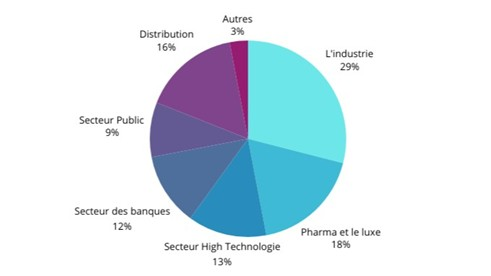
\includegraphics[width=0.85\textwidth]{figures/secteurs d'activité du groupe.jpg}
}{%
  \fbox{\parbox[c][3.5cm][c]{0.85\linewidth}{\centering \small Secteurs d'activit\'e du groupe VISEO\\(ajoutez figures/secteurs d'activit\'e du groupe.jpg)}}%
}
\caption{Secteurs d'activit\'e du groupe VISEO}
\label{fig:secteurs-activite}
\end{figure}

\subsection{Localisation et \'evolution}\label{ch1:localisation}

Depuis sa fondation en 1999, VISEO a connu une croissance soutenue, combinant cr\'eation organique,
d\'eveloppement de nouveaux services et acquisition d'activit\'es compl\'ementaires. La soci\'et\'e a construit
un projet collectif rassemblant une vari\'et\'e d'expertise, impliquant des dirigeants, des consultants
et des sp\'ecialistes techniques dans le d\'eveloppement d'une strat\'egie fond\'ee sur la conviction que
la technologie est un levier primordial de la transformation et de l'innovation.

Aujourd'hui, VISEO dispose d'une pr\'esence strat\'egique sur plus de 5 continents, avec des bureaux
localis\'es en France, Espagne, Portugal, Am\'erique, \'Etats-Unis, Chili, R\'epublique dominicaine, Panama,
Costa Rica, Singapour, Hong Kong, Indon\'esie, Philippines et Australie. La figure ci-dessous illustre
cette implantation mondiale.

\begin{figure}[h!]
\centering
\IfFileExists{figures/presence mondiale du groupe viseo.png}{%
	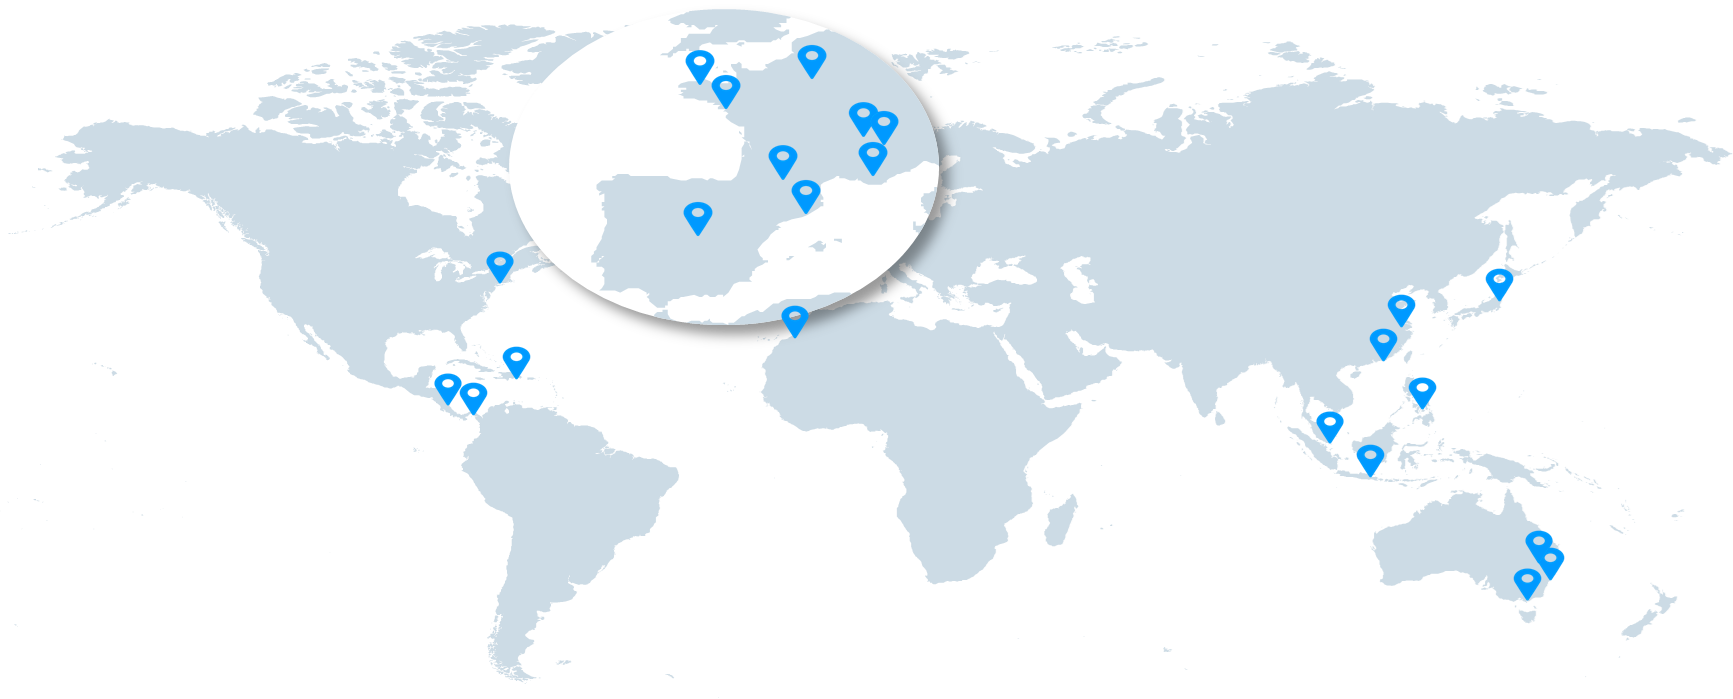
\includegraphics[width=0.92\textwidth]{figures/presence mondiale du groupe viseo.png}
}{%
	\fbox{\parbox[c][3cm][c]{\linewidth}{\centering \small Pr\'esence mondiale du groupe VISEO\\(ajoutez figures/presence mondiale du groupe viseo.png)}}
}
\caption{Pr\'esence mondiale du groupe VISEO}
\label{fig:presence-mondiale}
\end{figure}

Les bureaux se situent notamment dans les villes suivantes : Paris, Lyon, Grenoble, Metz, Nantes,
Toulouse, Aix-en-Provence, Madrid, Barcelone, Grenade, New York, Cuauht\'emoc, Hong Kong,
Shangha\"\i, Singapour, Tokyo, Sydney, Melbourne, Brisbane, Philippines, Indon\'esie, Panama,
Costa Rica et R\'epublique Dominicaine.

\subsection{Domaines d'expertise}\label{ch1:domaines}

VISEO a d\'evelopp\'e au fil des ann\'ees une expertise multidisciplinaire couvrant l'ensemble
du cycle de vie des syst\`emes d'information d'entreprise. Son positionnement repose sur
la capacit\'e \`a combiner des comp\'etences fonctionnelles pointues avec une ma\^itrise
technique des plateformes technologiques leaders du march\'e. La figure ci-dessous
synth\'etise les principaux domaines dans lesquels VISEO intervient.

\begin{figure}[h!]
\centering
\IfFileExists{figures/domaines de VISEO.jpg}{%
  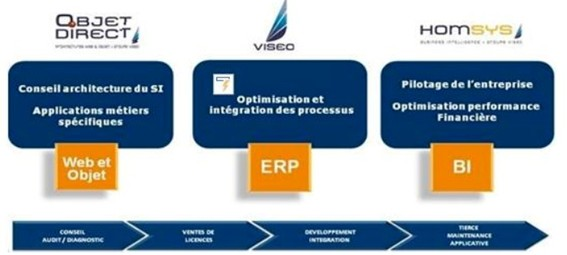
\includegraphics[width=0.88\textwidth]{figures/domaines de VISEO.jpg}
}{%
  \fbox{\parbox[c][3.5cm][c]{0.88\linewidth}{\centering \small Domaines d'expertise de VISEO\\(ajoutez figures/domaines de VISEO.jpg)}}%
}
\caption{Domaines d'expertise du groupe VISEO}
\label{fig:domaines-viseo}
\end{figure}

Ces domaines se d\'eclinent comme suit :

\begin{itemize}[label=\textbullet, itemsep=0.2em]
	\item \textbf{Syst\`emes d'information ERP} : Impl\'ementation, param\'etrage et maintenance
	      de solutions SAP et Microsoft Dynamics, couvrant l'ensemble des processus m\'etier
	      (achats, logistique, finance, production).
	\item \textbf{Digital \& Experience} : Conception d'interfaces utilisateur modernes,
	      applications mobiles et portails collaboratifs pour acc\'el\'erer la transformation
	      num\'erique des entreprises.
	\item \textbf{Cloud computing} : Migration vers des architectures cloud r\'esilientes
	      (Azure, AWS, SAP BTP) et optimisation des co\^uts d'infrastructure.
	\item \textbf{Data \& Intelligence artificielle} : Exploitation de la donn\'ee pour
	      g\'en\'erer des insights strat\'egiques, d\'eploiement de mod\`eles d'IA et
	      construction de tableaux de bord analytiques (Power BI, SAP Analytics Cloud).
	\item \textbf{Process \& Organisation} : Conseil en r\'eingenicerie des processus m\'etier,
	      gestion du changement et accompagnement des \'equipes lors des projets de transformation.
	\item \textbf{Cybersécurité et conformité} : Mise en place de dispositifs de s\'ecurit\'e
	      des syst\`emes d'information et accompagnement \`a la conformit\'e r\'eglementaire
	      (RGPD, normes sectorielles).
\end{itemize}

\subsection{Chiffres cl\'es}\label{ch1:chiffres}

VISEO, avec plus de \textbf{2\,500 collaborateurs} actuels, maintient une politique de recrutement
dynamique dans le but de former continuellement ses \'equipes, assurant ainsi une expertise constante
dans les technologies de pointe et les bonnes pratiques, \`a la fois dans le domaine informatique
et sectoriel.

En 2021, l'entreprise a enregistr\'e un \textbf{chiffre d'affaires de 265 millions d'euros}.
Cette croissance soutenue s'inscrit dans une trajectoire ininterrompue de 23 ans. En 2019,
VISEO avait d\'ej\`a r\'ealis\'e un chiffre d'affaires de \textbf{220 millions d'euros}, employant
alors \textbf{2\,200 salari\'es}.

Avec un chiffre d'affaires atteignant \textbf{358 millions d'euros} et un effectif de
\textbf{3\,000 collaborateurs} \`a la fin de l'ann\'ee 2023, VISEO consolide sa position sur
le march\'e. Organis\'ee autour de \textbf{six Business Units}, VISEO propose une gamme compl\`ete
de services, du conseil en amont des projets \`a l'optimisation des processus, en passant par
l'int\'egration, la maintenance et le d\'eveloppement de solutions m\'etiers verticales adapt\'ees
\`a divers secteurs d'activit\'e.

L'objectif principal de VISEO est d'accompagner ses clients dans leurs projets informatiques,
en fournissant une expertise technique, fonctionnelle et m\'etier pour optimiser les processus
et am\'eliorer les performances globales.

\vspace{0.3cm}

\begin{table}[h!]
\centering
\renewcommand{\arraystretch}{1.6}
\setlength{\tabcolsep}{14pt}
\renewcommand{\tabularxcolumn}[1]{m{#1}}
\rowcolors{3}{RoyalBlue!7}{white}
\begin{tabularx}{\textwidth}{>{\bfseries\color{MidnightBlue}\raggedright\arraybackslash}m{4.5cm} >{\centering\arraybackslash}X >{\centering\arraybackslash}X >{\centering\arraybackslash}X}
\toprule
\rowcolor{RoyalBlue!65}
\textcolor{white}{\textbf{Indicateur}} & \textcolor{white}{\textbf{2019}} & \textcolor{white}{\textbf{2021}} & \textcolor{white}{\textbf{2023}} \\
\midrule
Chiffre d'affaires & 220 M€ & 265 M€ & 358 M€ \\
Effectif & 2\,200 & 2\,500 & 3\,000 \\
\bottomrule
\end{tabularx}
\caption{\'Evolution des chiffres cl\'es du groupe VISEO (2019--2023)}
\label{tab:chiffres-viseo}
\end{table}

\vspace{0.4cm}

Les figures ci-dessous illustrent graphiquement cette trajectoire de croissance, en mettant
en \'evidence l'\'evolution du chiffre d'affaires et celle du nombre de collaborateurs sur
la p\'eriode r\'ecente.

\begin{figure}[h!]
\centering
\begin{minipage}[t]{0.48\textwidth}
\centering
\IfFileExists{figures/Chiffre d'affaires.jpg}{%
  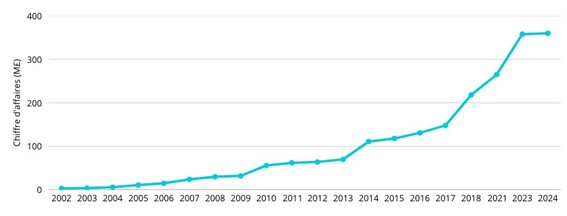
\includegraphics[width=\textwidth]{figures/Chiffre d'affaires.jpg}
}{%
  \fbox{\parbox[c][3.5cm][c]{\linewidth}{\centering \small \'Evolution du chiffre d'affaires\\(ajoutez figures/Chiffre d'affaires.jpg)}}%
}
\vspace{0.2cm}
{\small\textit{(a) \'Evolution du chiffre d'affaires (M€)}}
\end{minipage}
\hfill
\begin{minipage}[t]{0.48\textwidth}
\centering
\IfFileExists{figures/Evolutions du nombre de collaborateurs.jpg}{%
  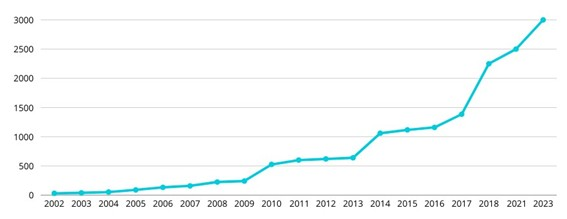
\includegraphics[width=\textwidth]{figures/Evolutions du nombre de collaborateurs.jpg}
}{%
  \fbox{\parbox[c][3.5cm][c]{\linewidth}{\centering \small \'Evolution des effectifs\\(ajoutez figures/Evolutions du nombre de collaborateurs.jpg)}}%
}
\vspace{0.2cm}
{\small\textit{(b) \'Evolution du nombre de collaborateurs}}
\end{minipage}
\caption{Croissance du groupe VISEO : chiffre d'affaires et effectifs}
\label{fig:croissance-viseo}
\end{figure}

\subsection{Filiale Casablancaise : VI ONE NORTH AFRICA}\label{ch1:filiale}

Depuis 2004, le groupe VISEO op\`ere au Maroc \`a travers sa filiale casablancaise,
\textbf{Vi-One North Africa}. Ce centre de services \textit{Nearshore} accompagne une
client\`ele diversifi\'ee, comprenant des entreprises fran\c{c}aises, am\'ericaines et
asiatiques, dans la r\'ealisation de leurs projets ou dans le cadre de contrats de
\textbf{Tierce Maintenance Applicative (TMA)}.

La position g\'eographique strat\'egique de Vi-One North Africa, \`a proximit\'e de
l'Europe et \`a mi-chemin entre les \'Etats-Unis et l'Asie, ainsi que sa localisation
au sein du plus grand parc d\'edi\'e aux services offshore du Maroc --- dot\'e
d'infrastructures de r\'eseau et de communication de pointe --- lui permettent de proposer
une gamme compl\`ete de services d'int\'egration d'ERP aux entreprises de la r\'egion.
Cette situation garantit \'egalement une proximit\'e et une r\'eactivit\'e constantes envers
sa client\`ele internationale.

Depuis sa cr\'eation, la filiale casablancaise a enregistr\'e une croissance continue, en
phase avec l'\'evolution du groupe. Elle offre d\'esormais une expertise pointue pour
r\'esoudre les probl\'ematiques li\'ees aux activit\'es ERP (telles que \textbf{SAP ECC},
\textbf{SAP S/4HANA} et \textbf{SAP Business One}), \`a l'optimisation de la cha\^ine
logistique, ainsi qu'aux d\'eveloppements web et objets connect\'es.

Gr\^ace au savoir-faire de son \'equipe hautement qualifi\'ee dans la mise en \oe uvre de
processus et de m\'ethodologies sp\'ecifiques \`a l'offshoring, la filiale a su s'adapter
aux besoins du march\'e et de ses clients, offrant ainsi des services de haute qualit\'e
et \`a forte valeur ajout\'ee \`a des co\^uts ma\^itris\'es. Avec plus de
\textbf{300 collaborateurs}, Vi-One North Africa constitue aujourd'hui un maillon
essentiel dans la strat\'egie de croissance internationale du groupe VISEO.

\vspace{0.4cm}

\begin{table}[h!]
\centering
\renewcommand{\arraystretch}{1.75}
\setlength{\tabcolsep}{14pt}
\renewcommand{\tabularxcolumn}[1]{m{#1}}
\rowcolors{3}{RoyalBlue!7}{white}
\begin{tabularx}{\textwidth}{>{\bfseries\color{MidnightBlue}\raggedright\arraybackslash}m{5.2cm} >{\raggedright\arraybackslash}X}
\toprule
\rowcolor{RoyalBlue!65}
\textcolor{white}{\textbf{\large Fiche d'identit\'e}} & \textcolor{white}{\textbf{\large VI-ONE North Africa}} \\
\midrule
NOM & VI-One North Africa \\
DATE DE CR\'EATION & 2004 \\
SECTEUR D'ACTIVIT\'E & Syst\`emes d'informations, ERP, Digital, Technologies, Process et Data \\
ADRESSE & Casanearshore Park, 1100 boulevard Al Qods, Shore 23, Plateau 701, Casablanca 20200, Maroc \\
T\'EL\'EPHONE & +212 5290-07346 \\
EFFECTIFS & +300 Collaborateurs \\
\bottomrule
\end{tabularx}
\caption{Fiche d'identit\'e de VI-ONE North Africa}
\label{tab:fiche-vione}
\end{table}

\vspace{0.4cm}

La figure suivante illustre la progression du nombre de collaborateurs au sein de
Vi-One North Africa, t\'emoignant de la croissance soutenue de la filiale depuis
sa cr\'eation.

\begin{figure}[H]
\centering
\IfFileExists{figures/Evolution du nombre de Collaborateurs au sein de VI-One North Africa.jpg}{%
  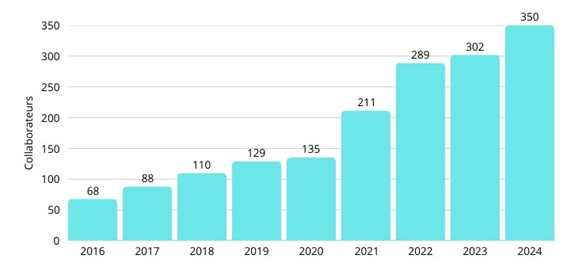
\includegraphics[width=0.85\textwidth]{figures/Evolution du nombre de Collaborateurs au sein de VI-One North Africa.jpg}
}{%
  \fbox{\parbox[c][3.5cm][c]{0.85\linewidth}{\centering \small \'Evolution des collaborateurs VI-One North Africa\\(ajoutez l'image correspondante)}}%
}
\caption{\'Evolution du nombre de collaborateurs au sein de VI-One North Africa}
\label{fig:collab-vione}
\end{figure}

\subsubsection{Organigramme}\label{ch1:organigramme}

L'organigramme de Vi-One North Africa refl\`ete une structure organisationnelle claire
et hi\'erarchis\'ee, con\c{c}ue pour assurer une coordination efficace entre les
diff\'erentes \'equipes et garantir la qualit\'e des prestations livr\'ees aux clients.
Chaque p\^ole dispose d'une responsabilit\'e bien d\'efinie, favorisant la sp\'ecialisation
et la r\'eactivit\'e face aux exigences des projets.

La filiale s'organise autour de plusieurs directions comp\'ementaires. La \textbf{Direction
G\'en\'erale} pilote la strat\'egie globale et assure la coordination avec le groupe VISEO.
Sous sa supervision, la \textbf{Direction Technique SAP} regroupe les consultants fonctionnels
et les d\'eveloppeurs ABAP charg\'es des projets d'int\'egration ERP. La \textbf{Direction
des Op\'erations} g\`ere les contrats de TMA et veille au respect des SLA clients.
Enfin, les fonctions support --- ressources humaines, finance et infrastructure IT ---
assurent le bon fonctionnement interne de la structure.

Cette organisation matricielle permet \`a Vi-One North Africa de mobiliser rapidement
les comp\'etences ad\'equates selon la nature et la complexit\'e de chaque mission client,
qu'il s'agisse d'un projet de d\'eploiement SAP S/4HANA, d'une maintenance applicative
ou d'un d\'eveloppement sp\'ecifique comme le pr\'esent projet de fin d'\'etudes.

\begin{figure}[H]
\centering
\IfFileExists{figures/organigramme-vione.jpg}{%
  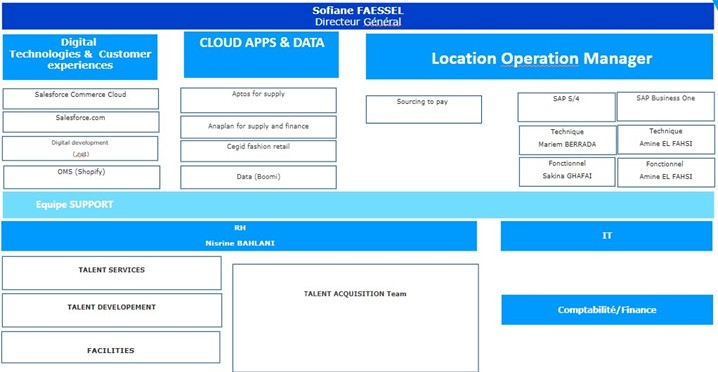
\includegraphics[width=0.92\textwidth]{figures/organigramme-vione.jpg}
}{%
  \fbox{\parbox[c][4cm][c]{0.92\linewidth}{\centering \small Organigramme de VI-ONE North Africa\\(ajoutez figures/organigramme-vione.jpg)}}%
}
\caption{Organigramme de VI-ONE North Africa}
\label{fig:organigramme-vione}
\end{figure}

\clearpage
\section{Cahier des charges}\label{ch1:cahier}

\subsection{Probl\'ematique}\label{ch1:problematique}

Dans le contexte actuel de digitalisation acc\'el\'er\'ee, la gestion des processus d'achats dans les
grandes entreprises demeure complexe et souvent fragment\'ee. Les relations fournisseurs traditionn
elles s'appuient sur des m\'ecanismes manuels, des \'echanges par email et des syst\`emes d'information
cloisonn\'es, g\'en\'erant :

\begin{itemize}[label=---, itemsep=0.15em]
	\item Des d\'elais de traitement allongés et une réactivité réduite
	\item Un manque de visibilité en temps r\'eel sur l'\'etat des commandes et des livraisons
	\item Des risques d'erreurs manuelles augment\'es et une tra\'cabilit\'e insuffisante
	\item Une exp\'erience utilisateur d\'egrad\'ee pour les fournisseurs
	\item Des lacunes dans la coordination entre les diff\'erentes \'etapes du processus
\end{itemize}

Ce constat a conduit l'entreprise partenaire \`a chercher une solution innovante permettant de
centraliser et d'automatiser la gestion des interactions avec ses fournisseurs, en exploitant les
capacit\'es avanc\'ees de la plateforme SAP.

\subsection{Objectifs}\label{ch1:objectifs}

L'objectif principal du projet est de concevoir et d\'eveloper un \textbf{Portail Fournisseur} offrant une
plateforme num\'erique centr\'alis\'ee et conviviale permettant aux fournisseurs de :

\begin{itemize}[label=\textbullet, itemsep=0.2em]
	\item \textbf{Consulter leurs commandes} en temps r\'eel avec une visibilité compl\`ete sur l'\'etat d'avancement
	\item \textbf{G\'erer les confirmations} de livraison et les r\'eceptions de mani\`ere efficace
	\item \textbf{Effectuer des op\'erations en masse} pour traiter plusieurs commandes simultan\'ement
	\item \textbf{Acc\'eder \`a des reportings d\'etaill\'es} pour analyser les tendances et performances
\end{itemize}

Les objectifs secondaires incluent l'am\'elioration de la satisfaction client, la r\'eduction des coûts
op\'erationnels et l'optimisation des flux logistiques.

\subsection{P\'erim\`etre}\label{ch1:perimetre}

Le projet couvre les aspects suivants :

\begin{itemize}[label=---, itemsep=0.15em]
	\item \textbf{Fonctionnalit\'es} : Consultation de commandes, confirmation/rejet, gestion en masse, reporting
	\item \textbf{Population cible} : Fournisseurs principaux et agences d'approvisionnement
	\item \textbf{Syst\`emes impliques} : SAP ECC, modules MM/CO, technologies RAP, SAPUI5
	\item \textbf{Infrastructure} : Environnement cloud SAP (le cas \'ech\'eant)
	\item \textbf{Donn\'ees trait\'ees} : Donn\'ees transactionnelles relatives aux commandes d'achat
\end{itemize}

Le p\'erim\`etre exclut les aspects avanc\'es de gestion de la supply chain, les pr\'evisions de demande
et les modules de facturation avanc\'ee, r\'eserv\'es \`a des phases ult\'erieures du projet.

\section{Gestion du projet}\label{ch1:gestion}

\subsection{M\'ethodologie adopt\'ee}\label{ch1:methodologie}
Le projet a \'et\'e pilot\'e suivant une approche \textbf{Agile}, se caract\'erisant par :

\begin{itemize}[label=---, itemsep=0.15em]
	\item \textbf{Sprints it\'eratifs} : D\'eveloppement en cycles courts (2-3 semaines) permettant une validation r\'eguli\`ere
	\item \textbf{R\'eunions de synchronisation} : Standup quotidiens et d\'ebriefing hebdomadaires avec l'\'equipe et le client
	\item \textbf{Feedback continu} : Validation des incr\'ements d\'evelopp\'es avec les parties prenantes
	\item \textbf{Adapt\'abilit\'e} : Capacit\'e \`a ajuster les priorit\'es en fonction des \'evolutions du contexte m\'etier
\end{itemize}

Cette approche a permis d'assurer un alignement r\'egulier avec les attentes du client et une r\'eduction
des risques li\'es aux \'evolutions de sp\'ecifications.

\subsection{Planification}\label{ch1:planification}

Le projet a \'et\'e structur\'e selon les phases suivantes :

\begin{itemize}[label=\textbullet, itemsep=0.2em]
	\item \textbf{Phase 1 - Initialisation (T1)} : D\'efinition des besoins, analyse de l'\'etat actuel et conception de l'architecture
	\item \textbf{Phase 2 - D\'eveloppement (T2-T3)} : Impl\'ementation des fonctionnalit\'es principales (consultation, confirmation, masse)
	\item \textbf{Phase 3 - Tests et affinement (T4)} : Validation fonctionnelle, tests de charge, correction des anomalies
	\item \textbf{Phase 4 - R\'eception et handover (T5)} : Pr\'eparation \`a la production, formation des utilisateurs, livraison
\end{itemize}

La dur\'ee totale du projet est estim\'ee \`a 5 mois, avec des jalons clairs et des d\'eliv\'erables
bien d\'efinis \`a chaque phase.

\section{Conclusion}\label{ch1:conclusion}

Le Chapitre 1 a pr\'esent\'e le contexte g\'en\'eral du projet, mettant en \'evidence l'importance stratégique
de la transformation num\'erique dans la gestion des relations fournisseurs. L'expertise reconnue de
VISEO, d\'eclin\'ee \`a travers ses domaines de comp\'etence et sa pr\'esence mondiale, la positionne comme
acteur id\'eal pour mener \`a bien ce projet ambitieux.

Le cahier des charges a \'etabli clairement la probl\'ematique, les objectifs poursuivis et le
p\'erim\`etre engag\'e. La m\'ethodologie agile retenue offre la flexibilit\'e n\'ecessaire pour r\'epondre aux
besoins en \'evolution, tandis que la planification structur\'ee garantit la d\'elivrance des r\'esultats dans
les d\'elais impartis.

Les chapitres suivants approfondiront l'\'etude de l'\'ecosyst\`eme SAP existant, la conception
d\'etaill\'ee de la solution, et les choix technologiques retenus pour mat\'erialiser cette vision.

\chapter{\'Etude et analyse de l'existant}\label{ch:existant}

\section{Introduction}\label{ch2:introduction}

Ce chapitre est consacré à l'étude approfondie de l'écosystème d'entreprise dans lequel s'inscrit notre projet.
Nous commencerons par une analyse générale des systèmes ERP, leurs rôles stratégiques et leurs bénéfices pour les organisations modernes.
Nous explorerons ensuite la plateforme SAP, leader incontesté du marché, en détaillant son positionnement, son architecture modulaire et ses capacités d'intégration.
Enfin, nous porterons notre attention particulière sur le module MM (Material Management), qui constitue le cœur fonctionnel de notre projet de portail fournisseur, en analysant ses processus, ses fonctionnalités clés et ses avantages concurrentiels.

\vspace{0.5cm}

\section{Les syst\`emes ERP : concepts et r\'ole strat\'egique}\label{ch2:erp}

\subsection{D\'efinition et concepts fondamentaux}\label{ch2:erp-def}

Un \textbf{Enterprise Resource Planning (ERP)}, ou \textbf{Progiciel de Gestion Intégré (PGI)} en français, est un système logiciel 
qui intègre et centralise l'ensemble des processus métier d'une organisation au sein d'une base de données unique et partagée. 
Contrairement aux systèmes traditionnels fragmentés, un ERP offre une vision holiste des activités de l'entreprise, permettant 
une meilleure coordination et une optimisation globale des opérations.

Les principaux modules d'un ERP typique incluent :

\begin{itemize}[label=\textbullet, itemsep=0.15em]
	\item \textbf{Finance et Comptabilité (FI/CO)} : Gestion des comptes, facturation, reporting financier
	\item \textbf{Ventes et Distribution (SD)} : Gestion des commandes clients, expéditions, facturation commerciale
	\item \textbf{Gestion des Matériaux (MM)} : Approvisionnement, gestion des stocks, gestion des fournisseurs
	\item \textbf{Production (PP)} : Planification de la production, gestion des ordres de fabrication
	\item \textbf{Gestion de Projets (PS)} : Suivi temporel et budgétaire des projects
	\item \textbf{Ressources Humaines (HR)} : Paie, gestion des talents, administration du personnel
	\item \textbf{Qualité (QM)} : Contrôle qualité et assurance qualité
\end{itemize}

\subsection{Rôle strat\'egique et bénéfices}\label{ch2:erp-role}

\begin{figure}[htbp]
\centering
\IfFileExists{figures/erp-diagram.png}{%
	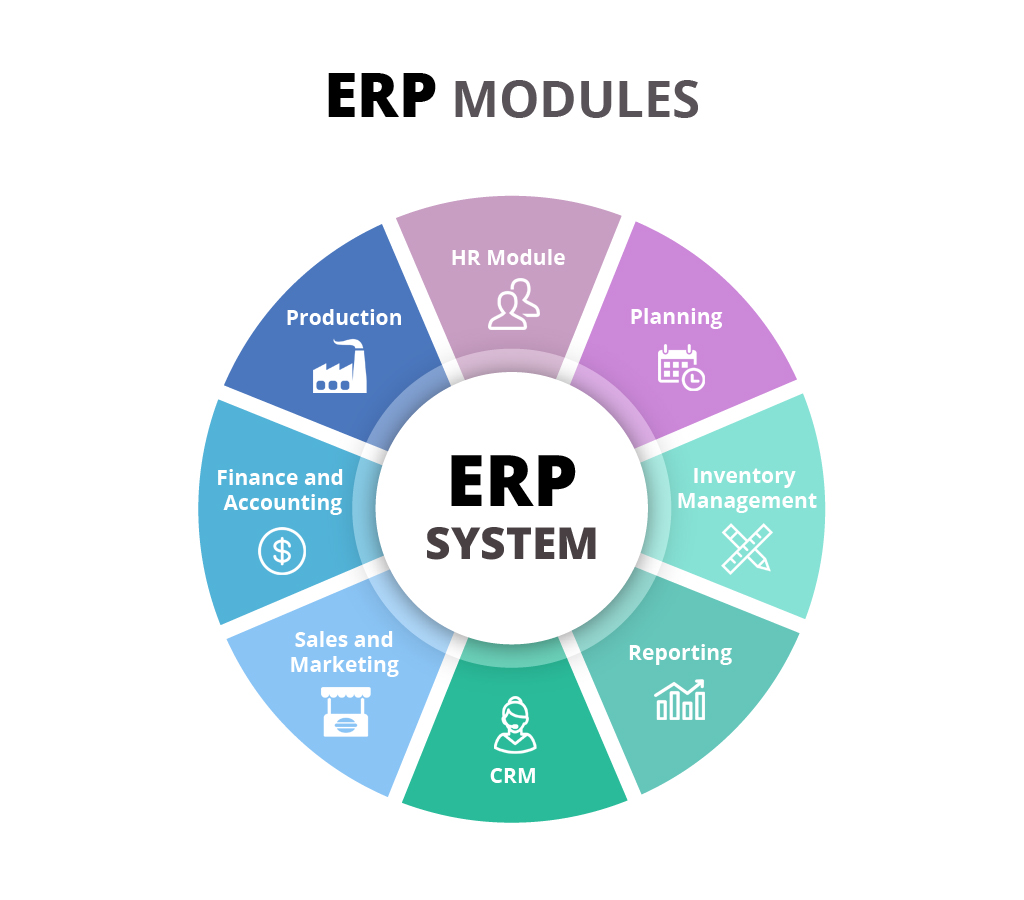
\includegraphics[width=0.8\textwidth]{figures/erp-diagram.png}
}{%
	\fbox{\parbox[c][2.5cm][c]{\linewidth}{\centering \small Diagramme des modules ERP intégrés\\(ajoutez figures/erp-diagram.png)}}
}
\caption{Architecture intégrée typique d'un système ERP}
\label{fig:erp-architecture}
\end{figure}

\vspace{0.3cm}

Les bénéfices stratégiques d'une implémentation ERP sont multiples :

\begin{enumerate}[label=(\roman*), itemsep=0.2em]
	\item \textbf{Visibilité en temps réel} : Les dirigeants disposent d'une vue d'ensemble consolidée de l'activité, permettant une prise de décision rapide et éclairée
	\item \textbf{Optimisation des processus} : L'automatisation des workflows réduit les délais et élimine les redondances
	\item \textbf{Réduction des coûts} : L'intégration diminue les erreurs manuelles, réduit les stocks et optimise les utilisation des ressources
	\item \textbf{Amélioration de la qualité données} : Une base de données unique garantit la cohérence et la fiabilité des informations
	\item \textbf{Scalabilité} : L'architecture modulaire permet une croissance adaptée aux besoins changeants de l'organisation
	\item \textbf{Conformité réglementaire} : Les outils de reporting intégrés facilitent le respect des normes légales et comptables
\end{enumerate}

Selon un rapport Gartner 2024, \textbf{87\% des entreprises classées Fortune 500} utilisent un système ERP pour leurs opérations critiques, 
soulignant l'importance stratégique incontournable de ces solutions dans le paysage technologique moderne.

\subsection{Évolution du marché des ERP}\label{ch2:erp-evolution}

Le marché des ERP a connu une transformation majeure au cours de la dernière décennie :

\begin{itemize}[label=---, itemsep=0.15em]
	\item \textbf{Migration vers le cloud} : Le passage progressif des solutions on-premise vers des environnements cloud SaaS
	\item \textbf{Intégration de l'IA et du Machine Learning} : Introduction de capacités prédictives et analytiques avancées
	\item \textbf{Mobilité et flexibilité} : Accès aux applications depuis n'importe quel terminal connecté
	\item \textbf{Micro-services et APIs} : Architecture modulaire permettant des intégrations plus faciles avec d'autres systèmes
	\item \textbf{Real-time analytics} : Reporting instantané et tableaux de bord dynamiques
\end{itemize}

\section{Pr\'esentation de SAP : leader mondial}\label{ch2:sap}

\subsection{Historique et position sur le marché}\label{ch2:sap-historique}

\begin{figure}[htbp]
\centering
\IfFileExists{figures/sap-logo.png}{%
	
\includegraphics[width=0.4\textwidth]{figures/sap-logo.png}
}{%
	\fbox{\parbox[c][1.8cm][c]{\linewidth}{\centering \small Logo SAP\\(ajoutez figures/sap-logo.png)}}
}
\caption{Logo SAP}
\label{fig:sap-logo}
\end{figure}

\vspace{0.3cm}

Fondée en 1972 en Allemagne, SAP (Systems, Applications, and Products in Data Processing) est la plus grande entreprise de 
logiciels métier au monde. Avec un siège social à Walldorf (Allemagne) et une présence dans \textbf{plus de 180 pays}, SAP 
s'est impérative comme solution de référence pour la gestion intégrée des processus métier.

\textbf{Chiffres clés de SAP} :

\vspace{0.5cm}

\begin{table}[h!]
\centering
\renewcommand{\arraystretch}{1.75}
\setlength{\tabcolsep}{14pt}
\renewcommand{\tabularxcolumn}[1]{m{#1}}
\rowcolors{3}{RoyalBlue!7}{white}
\begin{tabularx}{\textwidth}{>{\bfseries\color{MidnightBlue}\raggedright\arraybackslash}m{5.2cm} >{\raggedright\arraybackslash}X}
\toprule
\rowcolor{RoyalBlue!65}
\textcolor{white}{\textbf{\large Indicateur}} & \textcolor{white}{\textbf{\large SAP SE}} \\
\midrule
FONDÉE & 1972, Walldorf, Allemagne \\
CHIFFRE D'AFFAIRES & 32 Md€ (2023) \\
EMPLOYÉS & Plus de 105\,000 collaborateurs \\
PRÉSENCE MONDIALE & Plus de 180 pays \\
PART DE MARCHÉ ERP & 24\% (leader mondial) \\
CLIENTS & Plus de 440\,000 entreprises \\
\bottomrule
\end{tabularx}
\caption{Chiffres clés de SAP SE}
\label{tab:sap-chiffres}
\end{table}

\vspace{0.5cm}

\subsection{Portefeuille de solutions SAP}\label{ch2:sap-solutions}

SAP propose un portefeuille complet de solutions couvrant l'ensemble des besoins métier :

\begin{itemize}[label=\textbullet, itemsep=0.2em]
	\item \textbf{SAP S/4HANA} : Solution de nouvelle génération exploitant la base de données SAP HANA ultra-rapide, optimisée pour l'analyse en temps réel
	\item \textbf{SAP SuccessFactors} : Plateforme de gestion des talents et du capital humain
	\item \textbf{SAP Ariba} : Suite de sourcing et d'approvisionnement
	\item \textbf{SAP Analytics Cloud} : Plateforme d'analyse et de business intelligence
	\item \textbf{SAP BTP} : Business Technology Platform pour les applications et intégrations custom
\end{itemize}

\subsection{Architecture modulaire et intégration SAP}\label{ch2:sap-architecture}

L'architecture de SAP se compose de modules fonctionnels hautement intégrés :

\begin{figure}[htbp]
\centering
\IfFileExists{figures/sap-modules.png}{%
	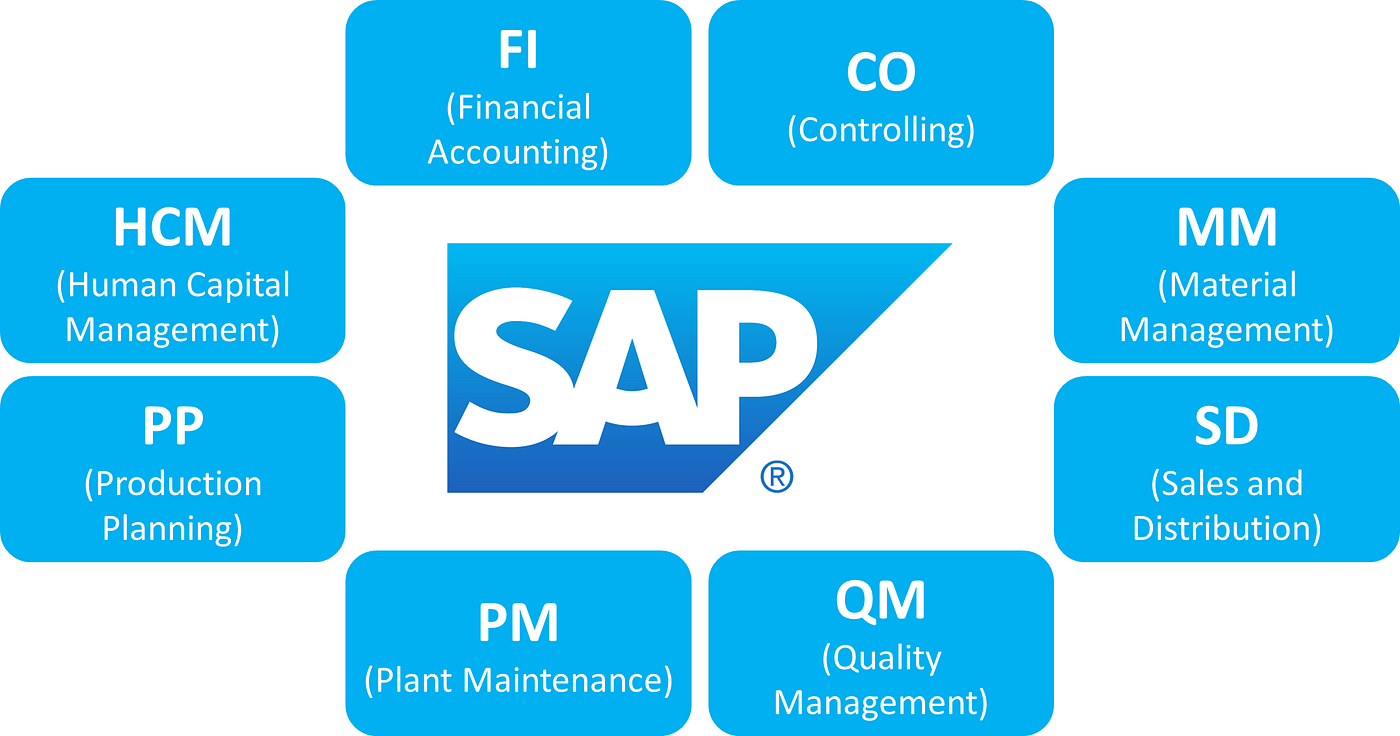
\includegraphics[width=0.85\textwidth]{figures/sap-modules.png}
}{%
	\fbox{\parbox[c][3cm][c]{\linewidth}{\centering \small Modules SAP et leurs intégrations\\(ajoutez figures/sap-modules.png)}}
}
\caption{Architecture des modules SAP et leurs intégrations}
\label{fig:sap-modules}
\end{figure}

\vspace{0.3cm}

La force majeure de SAP réside dans l'intégration native entre ses modules. Par exemple :

\begin{itemize}[label=---, itemsep=0.15em]
	\item Une \textbf{commande d'achat créée dans MM} alimente automatiquement les modules SD et FI
	\item Une \textbf{réception de marchandise} déclenche synchronisation les mouvements de stocks et les entrées comptables
	\item Un \textbf{ordre de fabrication en PP} consume automatiquement les matériaux du stock géré par MM
	\item Les \textbf{données HR} permettent l'allocation automatique des coûts aux centres de coûts
\end{itemize}

Cette intégration élimine les besoins de synchronisation manuelle et garantit la cohérence données à travers l'organisation.

\section{Le module MM : cœur de la gestion des matériaux}\label{ch2:mm}

\subsection{Présentation générale du module MM}\label{ch2:mm-presentation}

Le module \textbf{Material Management (MM)} de SAP est spécialisé dans la gestion complète du cycle de vie des matériaux, 
de l'approvisionnement jusqu'à la consommation. C'est un composant essentiel de tout système SAP, impactant les chaînes 
logistiques et les opérations de la majorité enterprises.

\textbf{Définition formelle} : SAP MM est un module intégré conçu pour gérer efficacement les processus d'approvisionnement, 
de gestion des stocks et de gestion des fournisseurs au sein d'une organisation. Il offre une plateforme centralisée pour 
contrôler et suivre toutes les activités liées aux matériaux, depuis leur acquisition jusqu'à leur consommation ou leur vente.

\subsection{Rôle critique dans les processus d'approvisionnement}\label{ch2:mm-role}

SAP MM revêt une importance capitale dans l'orchestration des processus d'approvisionnement et de gestion des stocks, 
offrant aux entreprises la capacité de :

\begin{enumerate}[label=\arabic*., itemsep=0.2em]
	\item \textbf{Planifier et exécuter l'approvisionnement} de matériaux, de biens et de services de manière optimisée
	\item \textbf{Suivre et contrôler les mouvements de stocks}, y compris les entrées, les sorties et les transferts
	\item \textbf{Gérer les fournisseurs}, évaluer leurs performances et maintenir des relations efficaces avec eux
	\item \textbf{Optimiser les processus métier} liés à la gestion des matériaux pour réduire les coûts et améliorer l'efficacité
	\item \textbf{Assurer la traçabilité complète} des articles du point d'approvisionnement à la consommation finale
	\item \textbf{Maintenir la disponibilité des stocks} tout en minimisant les ruptures et les surstock
\end{enumerate}

\subsection{Fonctionnalités clés du module MM}\label{ch2:mm-fonctionnalites}

\subsubsection{Gestion des approvisionnements}\label{ch2:mm-approv}

Le processus d'approvisionnement dans SAP MM comprend plusieurs étapes critiques :

\begin{itemize}[label=\textbullet, itemsep=0.15em]
	\item \textbf{Demande d'achat (Purchase Request)} : Les utilisateurs créent des demandes pour spécifier les articles nécessaires et les quantités requises demandées
	\item \textbf{Appel d'offres (RFQ)} : Processus de demande de devis auprès de multiples fournisseurs pour obtenir les meilleures conditions
	\item \textbf{Création de commandes d'achat (PO)} : Sur la base des demandes d'achat validées, les approvisionneurs créent des commandes formelles
	\item \textbf{Suivi des livraisons} : Tracking de l'état des commandes (non livrée, partiellement livrée, complètement livrée)
	\item \textbf{Réception de marchandises (GR)} : Enregistrement des entrées de matériel en utilisant des documents de réception standardisés
	\item \textbf{Facturation} : Rapprochement entre la commande, la réception et la facture fournisseur (three-way matching)
\end{itemize}

\begin{figure}[htbp]
\centering
\IfFileExists{figures/sap-mm-procurement.png}{%
	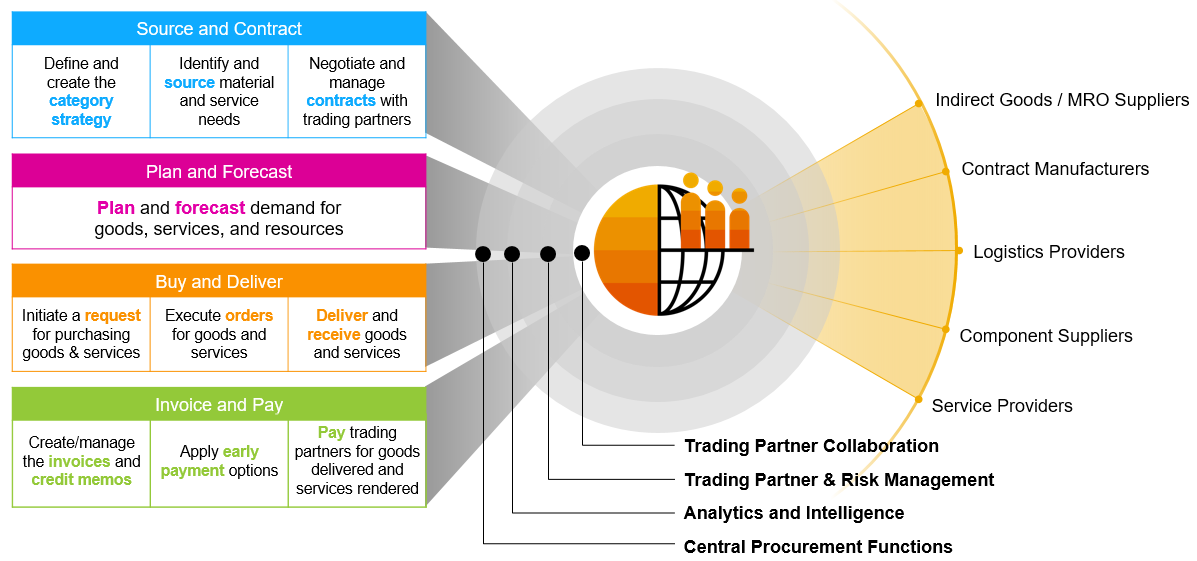
\includegraphics[width=0.8\textwidth]{figures/sap-mm-procurement.png}
}{%
	\fbox{\parbox[c][2.3cm][c]{\linewidth}{\centering \small Processus d'approvisionnement SAP MM\\(ajoutez figures/sap-mm-procurement.png)}}
}
\caption{Flux du processus MM}
\label{fig:sap-mm-procurement}
\end{figure}

\vspace{0.3cm}

\subsubsection{Gestion des stocks}\label{ch2:mm-stocks}

La fonction de gestion des stocks de SAP MM offre aux entreprises la capacité de surveiller et de contrôler de manière précise 
tous les flux de stocks. Les fonctionnalités clés comprennent :

\begin{itemize}[label=---, itemsep=0.15em]
	\item \textbf{Contrôle des mouvements de stocks} : SAP MM enregistre et suit les mouvements, permettant une traçabilité exhaustive
	\item \textbf{Valorisation stocks} : Évaluation selon différentes méthodes (coût moyen pondéré, coût standard, FIFO, LIFO)
	\item \textbf{Gestion multi-dépôts} : Suivi des stocks répartis dans plusieurs magasins et localisations
	\item \textbf{Contrôle d'accès} : Attribution des articles aux différents centres de coûts et domaines d'activité
	\item \textbf{Lot tracking} : Traçabilité complète des articles par lot, numéro de série ou date de fabrication
	\item \textbf{Analyse ABC} : Classification des matériaux pour optimiser le stockage et les commandes
\end{itemize}

\subsubsection{Gestion des fournisseurs}\label{ch2:mm-fourni}

SAP MM intègre une gestion complète du cycle de vie des relations fournisseurs :

\begin{itemize}[label=\textbullet, itemsep=0.2em]
	\item \textbf{Données fournisseurs centralisées} : Enregistrement et gestion des informations (coordonnées, conditions commerciales)
	\item \textbf{Évaluation des performances} : Suivi des KPIs fournisseurs (délai de livraison, qualité, conformité)
	\item \textbf{Gestion des risques} : Identification et mitigation des risques de rupture d'approvisionnement
	\item \textbf{Stratégie d'approvisionnement} : Consolidation des commandes, négociation des contrats cadres
	\item \textbf{Certification des fournisseurs} : Gestion des statuts de certification et de qualification
	\item \textbf{Analyse des dépenses} : Reporting détaillé pour identifier les opportunités d'optimisation
\end{itemize}

\subsection{Intégration avec les autres modules SAP}\label{ch2:mm-integration}

L'intégration entre SAP MM et les autres modules est essentielle pour une gestion complète des processus métier :

\subsubsection{Integration MM <-> SD (Ventes et Distribution)}\label{ch2:mm-int-sd}

\begin{itemize}[label=---, itemsep=0.15em]
	\item Les \textbf{commandes clients créées en SD} sont liées aux matériaux gérés en MM
	\item Les \textbf{stocks disponibles en MM} limitent la disponibilité promise aux clients en SD
	\item Les \textbf{livraisons de matériel} en MM impactent directement la satisfaction client en SD
	\item La \textbf{gestion de stock centralisée} assure une visibilité globale pour les deux modules
\end{itemize}

\subsubsection{Intégration MM <-> PP (Production)}\label{ch2:mm-int-pp}

\begin{itemize}[label=---, itemsep=0.15em]
	\item Les \textbf{ordres de fabrication} créés en PP consomment automatiquement les composants du stock MM
	\item Les \textbf{plannings de production} de PP alimentent les besoins en matières premières pour MM
	\item La \textbf{gestion des rebuts} est coordonnée entre les deux modules
	\item Les \textbf{stocks intermédiaires} sont suivis en MM pour l'optimisation de la production
\end{itemize}

\subsubsection{Intégration MM <-> FI (Finance)}\label{ch2:mm-int-fi}

\begin{itemize}[label=\textbullet, itemsep=0.2em]
	\item Les \textbf{valuations de stocks} générées en MM impactent le bilan comptable en FI
	\item Les \textbf{factures fournisseurs} de MM créent automatiquement les écritures comptables en FI
	\item Les \textbf{charges liées aux stocks} sont allocées aux bons comptes analytiques
	\item Les \textbf{rapprochements trois sens} (PO, GR, Invoice) assurent la sincérité comptable
\end{itemize}

Cette synchronisation garantit une visibilité en temps réel, réduit les erreurs et optimise les processus, 
entraînant une efficacité opérationnelle accrue et des coûts considérablement diminués.

\subsection{Avantages stratégiques de SAP MM}\label{ch2:mm-avantages}

\subsubsection{Amélioration de la visibilité et du contrôle}\label{ch2:mm-visibilite}

SAP MM offre une \textbf{visibilité en temps réel} sur l'ensemble du cycle de vie des matériaux, depuis leur commande 
jusqu'à leur utilisation ou leur vente. Les entreprises peuvent :

\begin{itemize}[label=---, itemsep=0.15em]
	\item Suivre chaque étape du processus d'approvisionnement avec un historique détaillé
	\item Identifier les goulots d'étranglement dans les flux logistiques
	\item Détecter et résoudre rapidement les problèmes potentiels
	\item Générer des alertes proactives pour les situations anormales (stock critique, délais de livraison dépassés)
\end{itemize}

\subsubsection{Optimisation des processus et réduction des coûts}\label{ch2:mm-optim}

En automatisant les processus d'approvisionnement, de gestion des stocks et de gestion des fournisseurs, SAP MM permet 
aux entreprises de :

\begin{itemize}[label=\textbullet, itemsep=0.2em]
	\item Réduire les délais de traitement des commandes (diminution moyenne de 30-40\%)
	\item Éliminer les inefficacités et minimiser les coûts liés à la gestion manuelle
	\item Identifier les fournisseurs les plus performants grâce à l'analyse comparative
	\item Optimiser les niveaux de stock pour minimiser le coût de détention (réduction moyenne de 15-25\%)
	\item Négocier des conditions d'achat avantageuses grâce aux données consolidées
\end{itemize}

\subsubsection{Prise de décisions basée sur des données en temps réel}\label{ch2:mm-decision}

Grâce aux fonctionnalités de reporting et d'analyse avancées de SAP MM, les entreprises disposent de :

\begin{itemize}[label=---, itemsep=0.15em]
	\item Données précises et actualisées sur l'activité d'approvisionnement et de gestion des stocks
	\item Tableaux de bord interactifs pour le monitoring continu des KPIs
	\item Prévisions fiables des besoins en matériaux basées sur des modèles analytiques
	\item Benchmarking des performances par rapport aux standards industrie
	\item Rapports détaillés pour une utilisation optimale des ressources
\end{itemize}

Ces avantages contribuent à une planification plus efficace, à une prise de décision stratégique mieux éclairée, 
et à un positionnement concurrentiel renforcé de l'entreprise.

\subsection{Cas d'usage réels et statistiques d'implémentation}\label{ch2:mm-casusage}

Plusieurs industries ont bénéficié significativement de l'implémentation de SAP MM :

\begin{itemize}[label=\textbullet, itemsep=0.2em]
	\item \textbf{Manufacturing} : Réduction du capital investi en stocks de 20-35\%, amélioration du taux de service de 10-15\%
	\item \textbf{Distribution \& Retail} : Amélioration de la rotation des stocks de 25-40\%, optimisation des coûts logistiques de 15-20\%
	\item \textbf{Automotive} : Synchronisation just-in-time à travers les chaînes de fournisseurs, réduction du défaut de 8-12\%
	\item \textbf{Pharmaceutique} : Conformité réglementaire renforcée, traçabilité complète des lots, réduction des recalls
	\item \textbf{Énergie \& Utilities} : Optimisation de la maintenance préventive, gestion des pièces de rechange, disponibilité accrue
\end{itemize}

Selon IDC (2023), \textbf{78\% des entreprises utilisant SAP MM} rapportent une amélioration significative 
de l'efficacité opérationnelle dans un délai de 18 mois suivant l'implémentation.

\subsection{Structure organisationnelle et entités du module MM}\label{ch2:mm-organisation}

SAP structure les données et les responsabilités à travers plusieurs niveaux organisationnels hiérarchisés, 
chacun correspondant à une entité métier distinct. Compren­dre cette architecture est essentiel pour configurer 
et exploiter correctement le module MM. Ces niveaux définissent les frontières des données, les permis­sions utilisateur, 
et la portée des transactions commerciales.

\subsubsection{Niveaux hiérarchiques organisationnels}\label{ch2:mm-org-niveaux}

\begin{itemize}[label=\textbullet, itemsep=0.2em]
	\item \textbf{Client} : Unité organisationnelle au sommet de la hiérarchie, représentant l'entité juridique principale. Chaque client possède son propre ensemble de données indépendantes et ses tables de configuration
	\item \textbf{Code d'entreprise (Company Code)} : Unité comptable autonome relevant d'un client, disposant de son propre compte de résultat et bilan. C'est la plus petite unité pour laquelle un ensemble complet d'enregistrements comptables peut être généré
	\item \textbf{Usine (Plant)} : Unité opérationnelle au sein d'une company code où se déploient les activités logistiques (fabrication, entrepôt, centre de distribution, site régional)
	\item \textbf{Emplacement de stockage (Storage Location)} : Niveau le plus détaillé de l'organisation, différenciant physiquement les zones de stockage au sein d'une usine. Les stocks y sont enregistrés individuellement
	\item \textbf{Organisation d'achat (Purchasing Organization)} : Entité responsable des activités d'approvisionnement et de négociation fournisseurs. Peut être centralisée au niveau client ou décentralisée par usine/company code
	\item \textbf{Groupe d'achat (Purchasing Group)} : Équipe ou personne responsable des achats quotidiens au sein d'une organisation d'achat
\end{itemize}

Cette architecture multi-niveaux permet une gestion granulaire des opérations tout en maintenant une vue consolidée au niveau du groupe.

\subsection{Transactions SAP et codes de transaction (T-codes)}\label{ch2:mm-transactions}

Une transaction SAP est un ensemble cohérent d'écrans, de programme et de règles métier permettant d'exécuter une opération commerciale spécifique dans le système. 
Chaque transaction est identifiée par un \textbf{code de transaction (T-code)} unique, permettant une navigation directe et rapide.

Les transactions du module MM englobent l'ensemble du cycle d'approvisionnement, de la planification initiale à la comptabilisation 
des factures. Elles offrent une interface standardisée pour garantir la cohérence des données et le respect des contrôles internes.

\subsection{Processus d'approvisionnement : taxonomie et stratégies}\label{ch2:mm-approv-process}

L'approvisionnement en matériaux et services est un processus fondamental qui doit être exécuté de manière optimale. 
Toute organisation acquiert des biens ou services pour répondre à ses besoins opérationnels, et SAP MM structure ce processus 
en deux catégories principales selon la nature et le traitement des acquisitions.

\subsubsection{Approvisionnement de base (Standard Procurement)}\label{ch2:mm-approv-base}

L'approvisionnement de base représente les acquisitions classiques de matériaux ou services, où l'entreprise devient propriétaire 
du bien au moment de la livraison. Les stratégies principales incluent :

\begin{itemize}[label=---, itemsep=0.15em]
	\item \textbf{Approvisionnement pour stocks} : Acquisition de matériaux conservés en inventaire pour une utilisation ultérieure
	\item \textbf{Approvisionnement pour consommation directe} : Achat de bien consommés immédiatement (fournitures, services)
	\item \textbf{Achats internes} : Transferts de matériaux entre entités du groupe
	\item \textbf{Achats externes} : Acquisitions auprès de fournisseurs tiers externes
\end{itemize}

L'équilibre optimal entre quantité, prix et délai est critique pour minimiser les coûts de stockage tout en assurant 
la continuité opérationnelle sans risque de pénurie.

\subsubsection{Approvisionnement spécialisé (Special Procurement)}\label{ch2:mm-approv-special}

Les stocks spécialisés désignent des biens dont l'entreprise ne détient pas la propriété directe mais qu'elle gère 
différemment des stocks conventionnels. Ces modalités offrent une flexibilité financière accrue et une gestion des risques optimisée :

\begin{itemize}[label=\textbullet, itemsep=0.2em]
	\item \textbf{Consignation} : Les matériaux restent propriété du vendeur jusqu'à leur utilisation effective par l'acheteur. L'entreprise ne paie que lorsque la consommation intervient
	\item \textbf{Service de prestataire (Third-Party Processing)} : Un fournisseur externe livre directement au client final sans que l'entreprise n'en prenne possession intermédiaire
	\item \textbf{Gestion de pipelines} : Pour les ressources livrées par infrastructure fixe (énergie, fluides), sans besoin de stockage physique
	\item \textbf{Emballages consignés} : Matériaux livrés dans des conteneurs réutilisables restant propriété du fournisseur
	\item \textbf{Sous-traitance} : L'entreprise fournit les composants à un prestataire qui effectue la fabrication ou transformation
\end{itemize}

Ces approches permettent d'optimiser la trésorerie, de réduire l'investissement en stocks et d'augmenter la flexibilité opérationnelle.

\subsection{Flux transactionnel complet du module MM}\label{ch2:mm-flux-transactionnel}

Le processus d'achat dans SAP MM constitue un flux structuré et intégré de transactions standard, enchaînées logiquement 
depuis l'identification du besoin jusqu'au règlement financier. Chaque transaction correspond à une étape métier distincte :

\subsubsection{Processus de création et gestion des demandes}\label{ch2:mm-flux-demandes}

\begin{itemize}[label=---, itemsep=0.15em]
	\item \textbf{ME51N (Demande d'achat)} : Permet aux utilisateurs de créer une demande interne quand un besoin est identifié. La demande peut être convertie en appel d'offres ou directement en commande selon le processus
	\item \textbf{ME41 (Appel d'offres / RFQ)} : Émet des demandes de devis auprès de fournisseurs pour évaluer les conditions tarifaires et sélectionner les meilleurs partenaires
	\item \textbf{ME61 (Évaluation des fournisseurs)} : Évalue les performances fournisseurs selon des critères (qualité, délais, respect des conditions) pour optimiser les sélections futures
\end{itemize}

\subsubsection{Processus de commande d'achat (Purchase Order)}\label{ch2:mm-flux-commande}

\begin{itemize}[label=\textbullet, itemsep=0.2em]
	\item \textbf{ME21N (Création de commande d'achat)} : Transaction principale créant une commande formelle à envoyer au fournisseur. Contient l'en-tête (données générales : fournisseur, conditions) et les lignes détaillant les articles
	\item \textbf{ME22N (Modification de commande d'achat)} : Permet de modifier une commande existante (quantités, prix, dates de livraison)
	\item \textbf{ME23N (Affichage de commande d'achat)} : Permet de consulter une commande et ses détails sans modification
\end{itemize}

Ces transactions sont le point de départ du cycle externe (interaction entreprise-fournisseur) et, dans le contexte 
d'un portail fournisseur, permettent aux vendeurs de confirmer ou rejeter les lignes de commande.

\subsubsection{Processus de réception et facturation}\label{ch2:mm-flux-reception}

\begin{itemize}[label=---, itemsep=0.15em]
	\item \textbf{MIGO (Entrée de marchandises / Goods Receipt)} : Enregistre la réception physique des produits livrés. L'entrée de stock est automatiquement reliée à la commande d'achat via son numéro
	\item \textbf{MIRO (Saisie de facture fournisseur / Invoice Receipt)} : Dernière étape du processus enregistrant la facture fournisseur. Vérifie le rapprochement trois sens (PO, réception, facture) avant déclenchement du paiement
\end{itemize}

Ce flux garantit un contrôle rigoureux des entrées, une correspondance comptable exacte et une maîtrise des dépenses.

\subsection{Structure et informations des commandes d'achat}\label{ch2:mm-purchase-order}

Une commande d'achat (Purchase Order - PO) est le document contractuel formalisant l'engagement d'achat. 
Elle se compose d'informations d'en-tête communes à toute la commande et de lignes détaillant chaque article acheté.

\subsubsection{Données d'en-tête de la commande}\label{ch2:mm-po-entete}

Stockées dans la table \textbf{EKKO}, les informations d'en-tête s'appliquent à l'intégralité de la commande :

\begin{itemize}[label=---, itemsep=0.15em]
	\item Numéro de commande (EBELN) : Identifiant unique de la commande dans le système
	\item Fournisseur (LIFNR) : Code du fournisseur sélectionné et ses coordonnées
	\item Organisation d'achat (EKORG) : Entité responsable de l'acte d'achat
	\item Groupe d'acheteurs (EKGRP) : Personne ou groupe responsable de la négociation
	\item Société (BUKRS) : Entité SAP qui émet la commande
	\item Date de création (AEDAT) et statut : Trace l'historique et l'état d'avancement
	\item Devise (WAERS) : Devise dans laquelle les prix sont exprimés
	\item Conditions de paiement (ZTERM) : Modalités de règlement négociées avec le fournisseur
\end{itemize}

\subsubsection{Données de lignes de la commande}\label{ch2:mm-po-lignes}

Stockées dans la table \textbf{EKPO}, les données de ligne (item) détaillent chaque article commandé :

\begin{itemize}[label=\textbullet, itemsep=0.2em]
	\item Numéro de ligne (EBELP) : Identifiant unique de la ligne au sein de la commande
	\item Code article (MATNR) : Référence du produit dans le système SAP
	\item Description (TXZ01) : Libellé commercial de l'article
	\item Quantité commandée (MENGE) et unité (MEINS) : Volume et unité de mesure
	\item Centre de livraison (WERKS) : Site destinataire de la livraison
	\item Date de livraison prévue (EINDT) : Date souhaitée pour la réception
	\item Prix unitaire (NETPR) et montant total : Informations de coût
	\item Quantités reçues/facturées : Suivi de l'avancement de la commande
\end{itemize}

Cette structure bi-niveaux permet un suivi granulaire par article et une traçabilité complète des engagements commerciaux.

\subsection{Architecture technique de SAP}\label{ch2:mm-arch-tech}

Sur le plan technique, SAP repose sur une \textbf{architecture client-serveur à trois tiers (3-tiers)}, séparant 
les responsabilités informatiques tout en assurant une grande flexibilité de déploiement. Chaque couche peut être 
hébergée sur une machine unique ou répartie sur plusieurs serveurs selon les besoins de performance.

\subsubsection{Couche de présentation}\label{ch2:mm-arch-pres}

\begin{itemize}[label=---, itemsep=0.15em]
	\item Interface utilisateur accessible via SAP GUI (client lourd) ou SAP Fiori (web moderne)
	\item Assure l'interaction entre l'utilisateur et le système
	\item Peut être déployée sur les postes utilisateurs ou en mode web centralisé
\end{itemize}

\subsubsection{Couche applicative}\label{ch2:mm-arch-app}

\begin{itemize}[label=\textbullet, itemsep=0.2em]
	\item Exécute la logique métier, les traitements et les programmes (notamment ABAP)
	\item Traite les transactions, applique les règles de gestion, effectue les calculs
	\item Peut être répartie sur plusieurs serveurs applicatifs pour distribuer la charge
	\item Gère la sécurité, les autorisations et la cohérence des données
\end{itemize}

\subsubsection{Couche base de données}\label{ch2:mm-arch-bdd}

\begin{itemize}[label=---, itemsep=0.15em]
	\item Contient les données persistantes de l'organisation (master data, transactions, historiques)
	\item Dans les versions modernes (S/4HANA), repose sur une base de données in-memory (SAP HANA) optimisée pour les traitements temps réel
	\item Offre une performance accrue, des capacités analytiques avancées et une scalabilité supérieure
\end{itemize}

\subsection{Organisation et paysage du système SAP}\label{ch2:mm-paysage-systeme}

Pour garantir la stabilité technique et l'intégrité des processus métier, SAP s'appuie sur une organisation 
rigoureuse des environnements système et des mécanismes de contrôle des changements.

\subsubsection{Paysage système (System Landscape)}\label{ch2:mm-landscape}

Le paysage recommandé comprend généralement trois environnements distincts :

\begin{itemize}[label=\textbullet, itemsep=0.2em]
	\item \textbf{DEV (Développement)} : Environnement dans lequel consultants et développeurs effectuent configurations et développements spécifiques. Point de départ des évolutions du système
	\item \textbf{QUAL (Qualité/Test)} : Environnement de test permettant de valider les évolutions dans des conditions proches de la production, avec jeux de données représentatifs
	\item \textbf{PROD (Production)} : Environnement en exploitation utilisé quotidiennement par les utilisateurs finaux. Le système le plus critique, où aucune modification directe ne doit être réalisée
\end{itemize}

Cette séparation assure une stabilité de production et permet des tests complets avant déploiement.

\subsubsection{Ordres de transport (Transport Orders - OT)}\label{ch2:mm-transport-orders}

Tout changement dans le système SAP (configuration, développement ABAP, corrections) est encapsulé dans un \textbf{ordre de transport} :

\begin{itemize}[label=---, itemsep=0.15em]
	\item Créé dans l'environnement DEV avec les modifications souhaitées
	\item Testé et validé en QUAL avec des scénarios d'utilisation réels
	\item Transporté en PROD après validation complète et approbation
	\item Fournit une traçabilité complète, une auditabilité et une cohérence des évolutions
\end{itemize}

Ce mécanisme assure que seules les évolutions validées et documentées accèdent à la production, minimisant 
les risques d'incidents et garantissant la reproductibilité des déploiements.

\section{Technologies SAP utilis\'ees}\label{ch2:tech}

\subsection{OData}\label{ch2:odata}

\textbf{OData (Open Data Protocol)} est un protocole standardisé pour l'échange de données via des services web REST. 
Dans le contexte SAP :

\begin{itemize}[label=---, itemsep=0.15em]
	\item Permet l'accès aux données SAP à travers des APIs standardisées et sécurisées
	\item Offre des capacités de filtrage, tri et pagination pour les requêtes de données
	\item Supporte les opérations CRUD (Create, Read, Update, Delete) sur les entités SAP
	\item Facilite l'intégration avec des applications tierces et des environnements hétérogènes
	\item Fournit des métadonnées (\$metadata) pour une découverte dynamique des données disponibles
\end{itemize}

\subsection{RAP}\label{ch2:rap}

\textbf{RESTful Application Programming (RAP)} est le framework moderne de SAP pour le développement d'applications 
d'entreprise :

\begin{itemize}[label=\textbullet, itemsep=0.2em]
	\item Basé sur une architecture de couches (Modeling Layer, Service Layer, Consumption Layer)
	\item Utilise Core Data Services (CDS) pour la modélisation déclarative des données et de la logique métier
	\item Généré automatiquement les services OData et les interfaces utilisateur Fiori
	\item Fournit les capacités built-in pour le versioning, les validations et les autorisations
	\item Accélère le développement et réduit la quantité de code personnalisé à maintenir
\end{itemize}

\subsection{SAPUI5}\label{ch2:sapui5}

\textbf{SAP UI5} est le framework JavaScript pour le développement d'interfaces utilisateur modernes et responsives :

\begin{itemize}[label=---, itemsep=0.15em]
	\item Framework riche pour construire des applications web d'entreprise
	\item Support complet de la responsive design (desktop, tablette, mobile)
	\item Composants visuels standardisés pour une cohérence UX à travers les applications SAP
	\item Intégration native avec les services OData pour la consommation des données
	\item Capacités avancées (binding de données, routing, internationalisation)
	\item Excellent performance et scalabilité pour les applications complexes
\end{itemize}

\section{Conclusion}\label{ch2:conclusion}

Ce chapitre a présenté une analyse exhaustive de l'écosystème ERP, du positionnement unique de SAP sur le marché, 
et des capacités spécialisées du module MM.

Les points clés retenus sont :

\begin{enumerate}[label=(\Alph*), itemsep=0.2em]
	\item Les systèmes ERP constituent une nécessité stratégique pour les entreprises modernes cherchant 
	à optimiser leurs opérations et réduire leurs coûts
	\item \textbf{SAP} s'affirme comme le leader mondial incontesté avec une part de marché de 24\% et une présence 
	établie chez 89\% des plus grandes entreprises mondiales
	\item Le module \textbf{MM} offre une gestion intégrée complète de la chaîne d'approvisionnement, 
	essentielle pour la compétitivité dans un environnement économique tendu
	\item L'intégration native entre MM et les autres modules SAP crée un écosystème puissant 
	qui élimine les silos fonctionnels et améliore la prise de décision
	\item Les technologies modernes (OData, RAP, SAPUI5) permettent le développement rapide 
	d'extensions et d'applications sur la plateforme SAP
	\item Les implémentations réussies de SAP MM génèrent un ROI significatif, 
	avec des améliorations mesurables dans les délais, les coûts et la qualité des services
\end{enumerate}

Cette connaissance approfondie du contexte technologique et métier forme la base solide 
sur laquelle repose la conception et le développement de notre portail fournisseur, 
sujet du chapitre suivant.

\chapter{Analyse et conception de la solution}\label{ch:analyse-conception}

\section{Introduction}\label{ch3:introduction}
Ce chapitre constitue le cœur méthodologique et conceptuel du projet de fin d'études. Il détaille le passage d'une problématique métier — les inefficacités et le manque de visibilité dans le cycle de confirmation des commandes abordés au chapitre précédent — à la conception d'une architecture logicielle aboutie, robuste et conforme aux standards de l'écosystème SAP S/4HANA. 

Dans le cadre de cette mission d'Assistance à la Maîtrise d'Ouvrage (AMOA), l'objectif ne s'est pas limité à la création d'une simple interface de consultation de données. La solution a été pensivement architecturée comme une plateforme d'interaction sécurisée, hautement performante, permettant à la fois le traitement unitaire et le traitement en masse (via Excel) des commandes d'achat. Parallèlement, elle devait offrir une visibilité analytique en temps réel aux départements achats et s'intégrer harmonieusement avec les technologies d'Intelligence Artificielle de pointe (SAP Joule). Les sections qui suivent exposent la démarche d'analyse, l'expression détaillée des exigences, la modélisation UML des processus, ainsi que les choix architecturaux décisifs qui structurent la solution.

\section{Démarche méthodologique et répartition des tâches}\label{ch3:demarche}
La conception d'une application transactionnelle et analytique de cette envergure nécessite une approche méthodologique rigoureuse pour garantir l'alignement avec les processus logistiques de l'entreprise. L'équipe projet a adopté une méthodologie Agile (Scrum), caractérisée par des itérations courtes (sprints) permettant des retours utilisateurs rapides et continus.

Sur le plan de l'organisation technique du développement, nous avons fait le choix stratégique d'une répartition des tâches basée sur l'approche du \textbf{Vertical Split} (découpage vertical), rompant avec le découpage horizontal classique par couches isolées (Base de données d'un côté, Backend au centre, Frontend de l'autre). 
Dans cette dynamique, chaque membre du binôme a pris l'entière responsabilité de fonctionnalités complètes, de bout en bout. Par exemple, lors de la conception de la fonctionnalité de gestion des rejets, l'intervenant en charge a modélisé les tables de journalisation personnalisées (comme \texttt{ZTPO\_REJECT\_LOG}), créé les vues \textit{Core Data Services} (CDS) correspondantes, implémenté le comportement métier transactionnel (via les \textit{Behavior Definitions} ABAP RAP), jusqu'à la projection de ces données sur l'interface graphique SAP Fiori. Cette responsabilisation complète a considérablement réduit les goulots d'étranglement lors des phases d'intégration et a permis de forger une vision globale et maîtrisée de l'architecture logicielle SAP.

\section{Ingénierie des exigences et spécifications}\label{ch3:analyse-besoins}

L'étape d'ingénierie des exigences permet de traduire les contraintes opérationnelles en spécifications logicielles précises. Suite à plusieurs ateliers d'expression de besoins avec les parties prenantes, le périmètre a été défini autour de deux axes : les fonctionnalités métiers directes et les contraintes techniques du système.

\subsection{Exigences fonctionnelles métiers}\label{ch3:besoins-f}
Les exigences fonctionnelles décrivent la capacité du système à répondre aux actions métier attendues par les acheteurs et les fournisseurs.

\begin{itemize}[label=-]
    \item \textbf{Visibilité dynamique et suivi centralisé :} Le portail doit fournir une vue unifiée et filtrable de l'ensemble des commandes d'achat (Purchase Orders) assignées à un fournisseur spécifique. L'interface doit exposer des indicateurs clés tels que le numéro de la commande, la date d'émission, les montants totaux, les devises, et surtout l'échéance de réponse. Le fournisseur doit également pouvoir explorer le détail d'une commande pour consulter les différentes lignes d'articles, les quantités requises et les adresses de livraison prévues.
    \item \textbf{Traitement unitaire et qualification des rejets :} Le système doit permettre au fournisseur de sélectionner individuellement une ligne de commande pour la confirmer ou la rejeter. Dans le cas d'un rejet, l'application doit imposer la sélection d'un motif clair et normé parmi une nomenclature préétablie (par exemple : produit définitivement indisponible, délai de production impossible, ou fin de contrat avec l'entreprise). Ce motif structuré est vital pour alimenter les statistiques de performance des fournisseurs.
    \item \textbf{Traitement en masse via tableur (Excel) :} Afin de respecter les contraintes de productivité des grands fournisseurs qui traitent plusieurs dizaines, voire centaines de références par jour, l'interface doit intégrer un mécanisme de traitement par lots. Le fournisseur doit pouvoir télécharger un modèle Excel, le compléter hors ligne, puis l'importer dans le système. L'application doit analyser le fichier, valider son intégrité, et appliquer massivement les statuts dans S/4HANA au sein d'une transaction unique pour éviter toute corruption des données.
    \item \textbf{Génération de la documentation formelle :} Le système doit inclure un moteur permettant la génération instantanée des bons de commande au format standardisé PDF, facilitant ainsi l'archivage ou l'impression physique par le fournisseur.
    \item \textbf{Pilotage Analytique Interactif (Dashboard) :} Les départements achats nécessitent des outils de pilotage visuels. Une page analytique (\textit{Analytical List Page}) doit être disponible, offrant des \textit{Visual Filters} (tels que des graphiques en anneau pour les statuts et des histogrammes pour les fournisseurs ou les motifs de rejet). Ces filtres visuels doivent permettre de découper et de filtrer dynamiquement les immenses volumes de données logistiques en quelques clics.
\end{itemize}

\subsection{Exigences non fonctionnelles et architecturales}\label{ch3:besoins-nf}
Pour assurer la fiabilité, la sécurité, et la maintenabilité à long terme de la plateforme, un cahier des charges technique strict a été dressé.

\begin{itemize}[label=-]
    \item \textbf{Sécurité, SSO et cloisonnement des données :} Étant exposé à des acteurs externes (les fournisseurs), le portail exige une authentification robuste (Single Sign-On). Il est impératif d'implémenter un contrôle d'accès au niveau de la base de données (Authorization Checks). Le système doit garantir un isolement strict des données : un fournisseur connecté ne doit sous aucun prétexte pouvoir requêter ou visualiser les données concurrentielles d'un autre fournisseur.
    \item \textbf{Traçabilité réglementaire (Audit Logs) :} Chaque modification d'état (qu'il s'agisse d'une confirmation ou d'un rejet) doit obligatoirement générer une entrée immuable dans une table de journalisation (Log Table). Ce registre doit conserver l'identifiant de l'utilisateur, l'horodatage exact, ainsi que la nature de l'altération pour répondre aux normes strictes des audits financiers et logistiques.
    \item \textbf{Cohérence technologique et modernité :} Le code résidant côté serveur doit rompre avec l'utilisation des anciennes BAPI (Business Application Programming Interfaces) monolithiques. La logique transactionnelle doit reposer exclusivement sur le modèle moderne SAP RAP (RESTful Application Programming), exposant des services standardisés et sécurisés.
    \item \textbf{Expérience Utilisateur (UX) :} L'interface doit respecter rigoureusement les directives de design de SAP Fiori Elements. Elle doit être \textit{Responsive} (parfaitement fonctionnelle sur ordinateur de bureau comme sur terminal mobile) et garantir des temps de chargement minimes.
\end{itemize}

\section{Modélisation des processus et Cas d'utilisation}\label{ch3:cas-util}
Le diagramme de cas d'utilisation ci-dessous englobe les périmètres d'interaction des différents acteurs avec le portail fournisseur. Il fait ressortir la séparation nette entre le traitement transactionnel (agir sur les données) et le traitement analytique (observer les données).

\begin{figure}[htbp]
\centering
\IfFileExists{figures/usecases-diagram.png}{%
    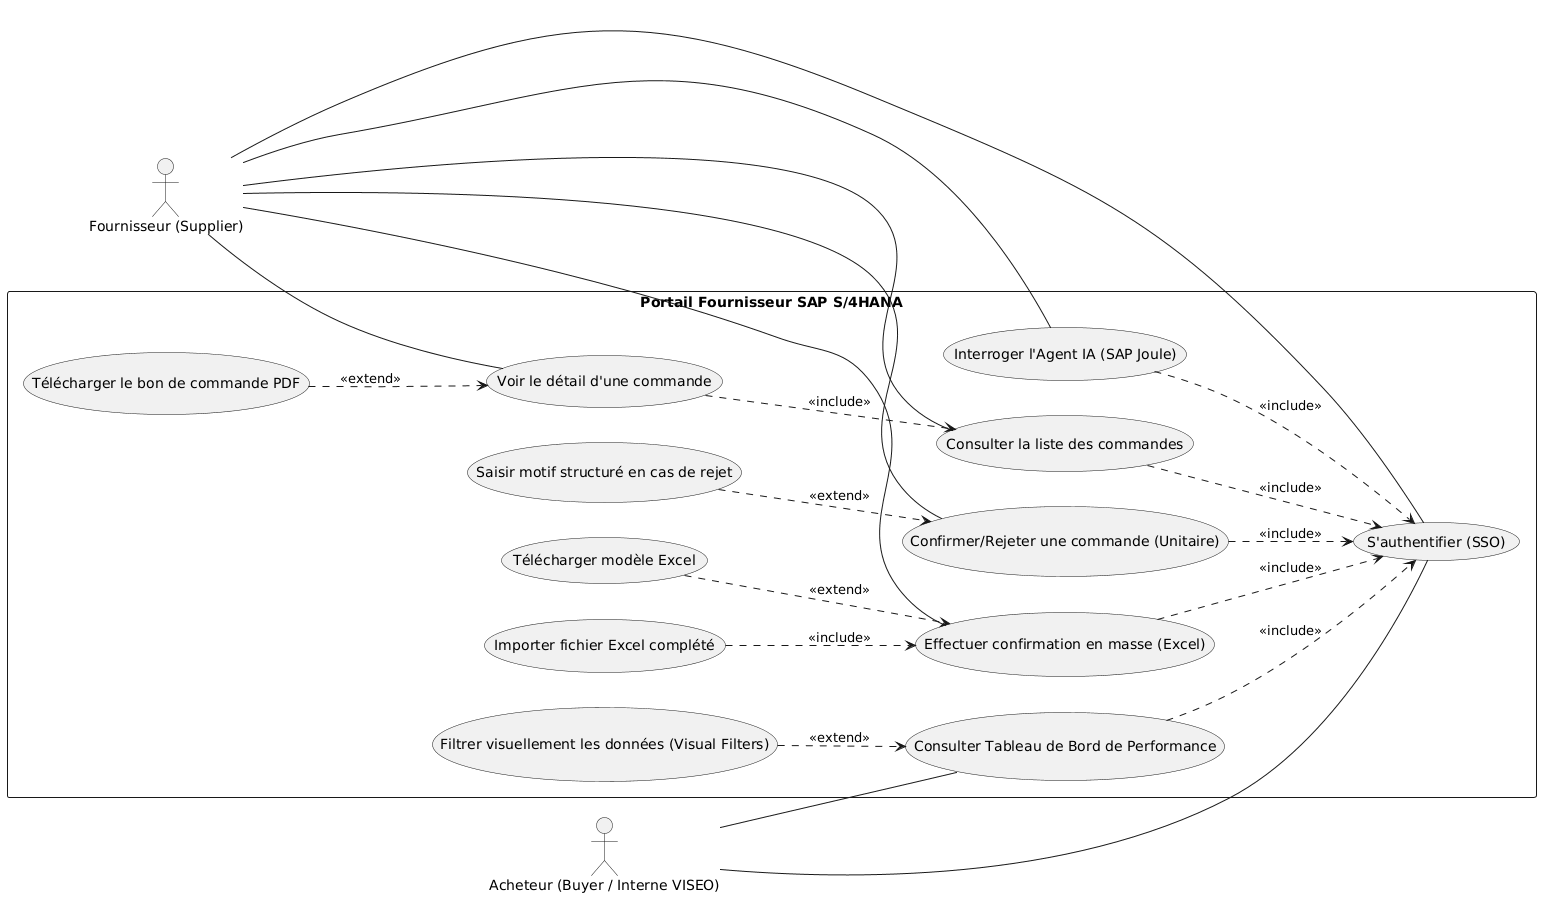
\includegraphics[width=0.9\textwidth]{figures/usecases-diagram.png}
}{%
    \fbox{\parbox[c][5cm][c]{0.9\linewidth}{\centering \small Diagramme global de Cas d'Utilisation\\(ajoutez figures/usecases-diagram.png)}}
}
\caption{Diagramme global des cas d'utilisation du portail fournisseur}
\label{fig:usecases}
\end{figure}

\section{Architecture globale et choix technologiques}\label{ch3:architecture}
La transition d'un ensemble de règles métiers vers une application fonctionnelle requiert une architecture solide. Pour s'affranchir des limitations historiques des ERP et s'aligner sur la stratégie orientée Cloud de SAP, nous avons conçu une architecture multiniveaux et hybride.

\textbf{La couche de persistance (Base de données S/4HANA)} \\
L'intégrité de la solution repose sur la base de données In-Memory SAP HANA. Plutôt que de manipuler directement les immenses tables standards des achats (telles que \texttt{EKKO} pour les en-têtes et \texttt{EKPO} pour les lignes), nous avons structuré l'accès aux données grâce aux \textit{Core Data Services} (CDS). Une pyramide de vues a été construite : des vues de base (Basic Views) extraient les données brutes, des vues composites effectuent les jointures complexes (avec les tables fournisseurs et nos tables personnalisées de logs), et enfin des vues de consommation (Consumption Views) annotent ces données pour définir la manière dont elles devront s'afficher sur l'écran final.

\textbf{La couche de Logique Métier (Modèle ABAP RAP)} \\
Pour garantir la cohérence des opérations transactionnelles (confirmation et rejet), nous nous appuyons sur l'architecture SAP RAP. Les règles d'entreprise sont encapsulées dans des "Behavior Definitions" et des "Behavior Pools" (Classes ABAP). Cela permet d'exécuter de puissantes validations avant même qu'une modification ne soit écrite en base. Cette couche est ensuite exposée sous la forme de services web modernes via le protocole \textbf{OData V4}, optimisé pour les opérations de mise à jour et d'insertion par lots (indispensable pour notre import Excel).

\textbf{Le défi du Dashboard Analytique et l'hybridation OData} \\
Lors de la conception du tableau de bord (Analytical List Page), nous avons fait face à une limite technique majeure du standard. Les \textit{Visual Filters} (graphiques agissant comme des filtres interactifs) dépendent du moteur analytique profond de SAP (le moteur BICS - Business Intelligence Consumer Services). Cependant, le protocole OData V4 ne supporte pas encore de manière optimale les requêtes BICS complexes nécessaires à ces graphiques. Plutôt que de sacrifier cette fonctionnalité métier cruciale, nous avons élaboré une architecture de contournement (\textit{bypass}) : le tableau de bord analytique a été isolé et exposé à travers une couche \textbf{OData V2} classique générée automatiquement via l'annotation \texttt{@OData.publish: true}, connectant directement le Frontend au moteur BICS. L'application est donc hybride, utilisant OData V4 pour la robustesse transactionnelle et OData V2 pour l'agilité analytique.

Pour illustrer l'organisation de ces différentes couches et leurs interactions via le réseau, le schéma suivant modélise l'architecture système globale :

\begin{figure}[htbp]
\centering
\IfFileExists{figures/architecture-layers.png}{%
    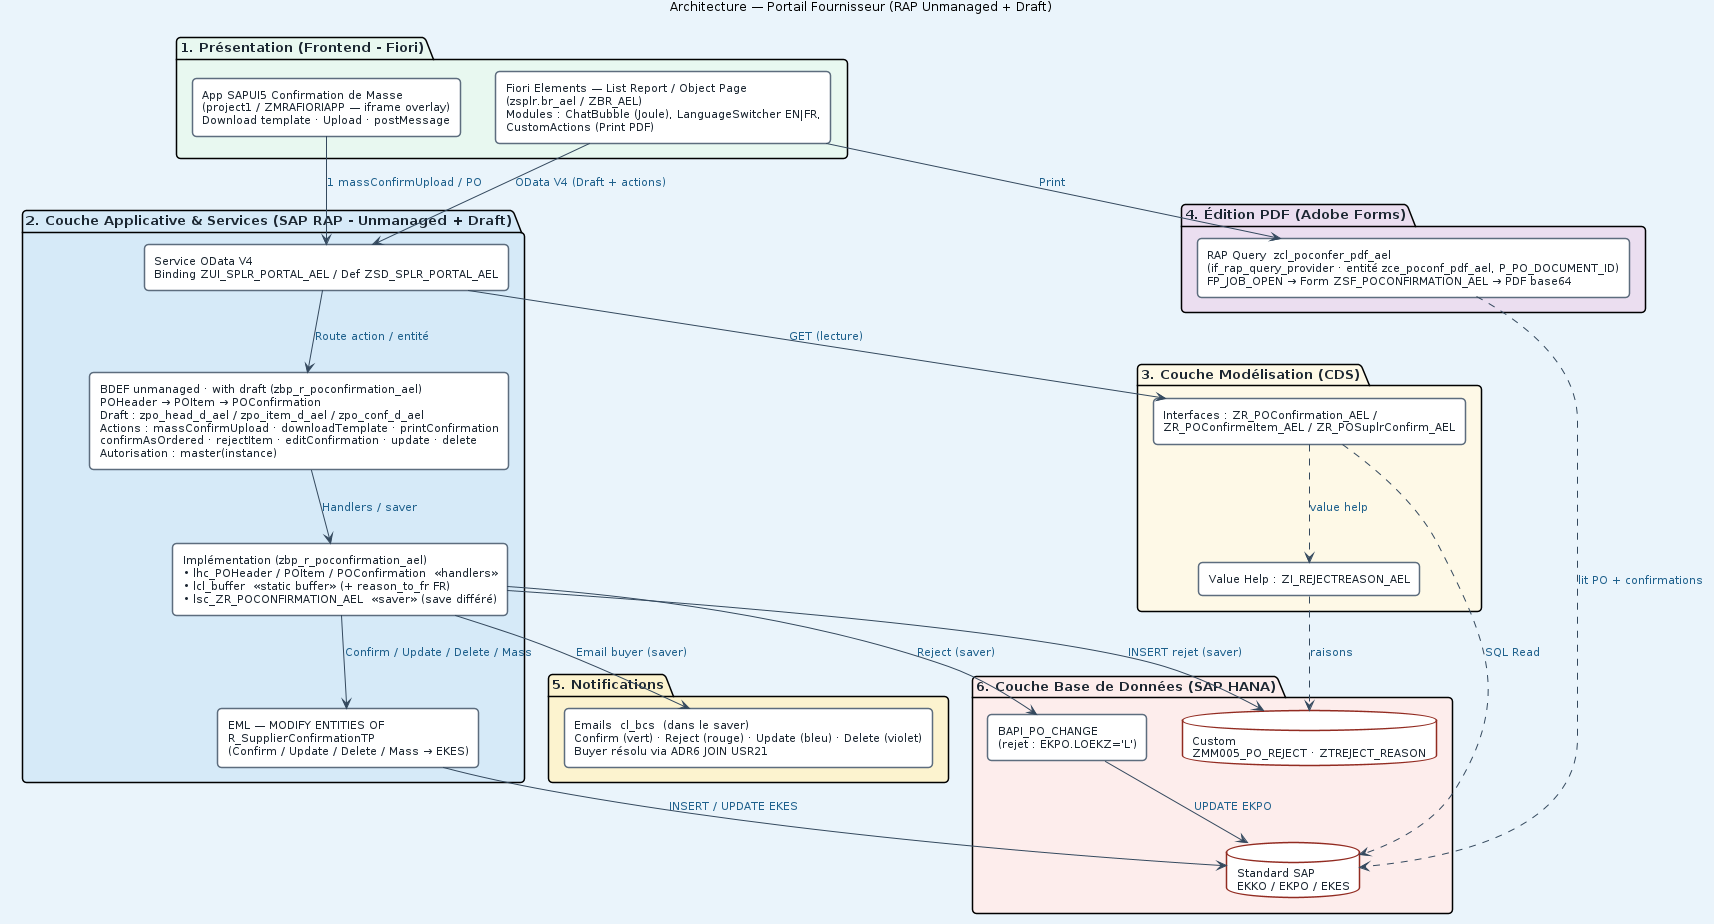
\includegraphics[width=0.9\textwidth]{figures/architecture-layers.png}
}{%
    \fbox{\parbox[c][5cm][c]{0.9\linewidth}{\centering \small Architecture en couches de la solution\\(ajoutez figures/architecture-layers.png)}}
}
\caption{Architecture en couches de la solution hybride (CDS, RAP, Fiori)}
\label{fig:architecture}
\end{figure}

\section{Conception détaillée et modélisation}\label{ch3:uml}
\subsection{Modèle de données}\label{ch3:diag-classes}
Le modèle relationnel est le cœur opérationnel de l'application. Il tisse les liens entre les éléments standards de SAP et nos propres développements. Outre les tables de commandes, nous avons modélisé des tables spécifiques pour gérer notre propre logique. Par exemple, la table \texttt{ZTPO\_REJECT\_LOG} a été conçue avec une clé étrangère pointant vers le numéro de ligne de la commande, et un champ associant explicitement le rejet à un motif normé de notre dictionnaire de données. Le diagramme de classes suivant expose ces entités, leurs attributs techniques (types et cardinalités) ainsi que les méthodes métiers qui leurs sont rattachées.

\begin{figure}[htbp]
\centering
\IfFileExists{figures/class-diagram.png}{%
    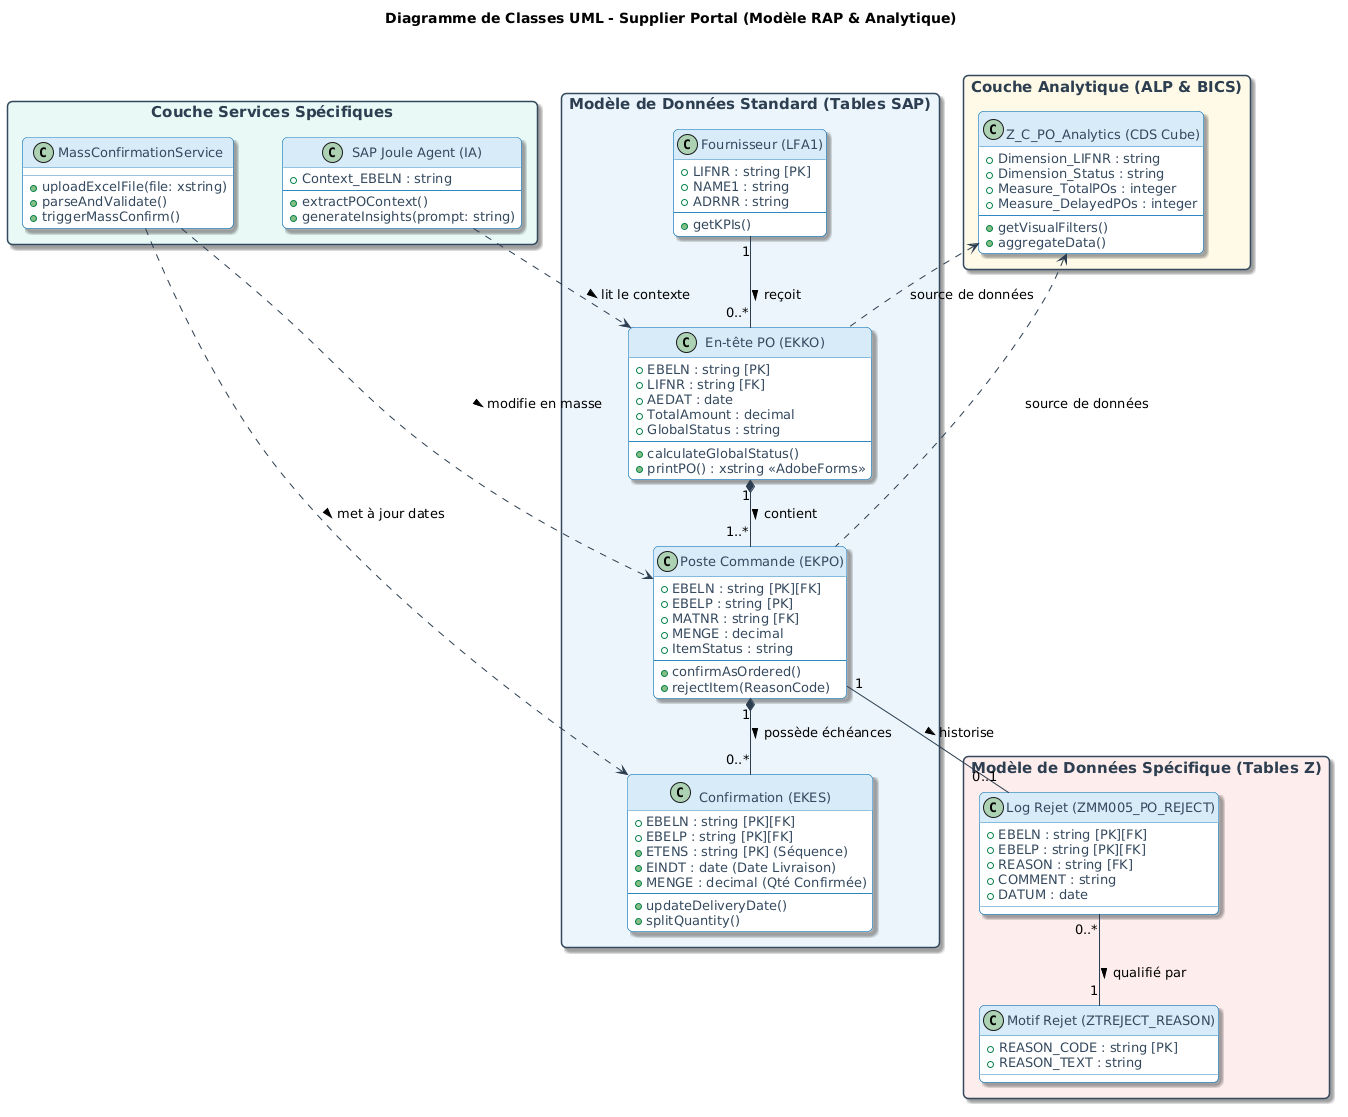
\includegraphics[width=0.9\textwidth]{figures/class-diagram.png}
}{%
    \fbox{\parbox[c][5cm][c]{0.9\linewidth}{\centering \small Diagramme de classes UML\\(ajoutez figures/class-diagram.png)}}
}
\caption{Diagramme de classes UML du modèle de données étendu}
\label{fig:classes}
\end{figure}

\subsection{Flux transactionnels et asynchronisme}\label{ch3:diag-sequences}
Comprendre le cheminement d'une information entre l'écran du fournisseur et la base de données est vital, particulièrement pour la fonctionnalité de confirmation en masse via fichier Excel, qui représente un défi technique en termes de synchronisation. 

Lorsqu'un fournisseur charge son fichier XLSX sur le portail, le processus s'initie intégralement côté client (Frontend). Une bibliothèque JavaScript (généralement \texttt{SheetJS} dans le contexte UI5) parse le fichier binaire localement et le transforme en un "Payload" JSON structuré. Cette charge utile est ensuite expédiée de manière asynchrone au backend S/4HANA via l'API OData V4. Le gestionnaire ABAP RAP réceptionne cette matrice, itère sur chaque ligne en mémoire, exécute les contrôles de sécurité (validation du fournisseur, existence de la commande, validité de la date), puis procède à un \textit{Commit} global dans la base de données. Enfin, il renvoie un code de statut HTTP avec un rapport détaillé des succès et erreurs éventuelles pour rafraîchir l'interface utilisateur. 

Ce dialogue complexe entre le navigateur, le serveur d'application, et la base de données est modélisé dans le diagramme de séquence ci-dessous :



\section{Stratégie d'automatisation et Agent IA (SAP Joule)}\label{ch3:ia-joule}
L'un des axes d'innovation majeurs de notre conception réside dans l'intégration de l'intelligence artificielle générative pour sublimer l'expérience utilisateur. L'objectif était de permettre au fournisseur d'interagir avec la masse de données ERP non plus via des menus complexes, mais par une simple conversation en langage naturel grâce à l'assistant natif \textbf{SAP Joule}.

L'architecture conceptuelle de cette interaction est inspirée des systèmes RAG (\textit{Retrieval-Augmented Generation}). Lorsqu'un fournisseur interroge Joule (par exemple : "Montre-moi un résumé de mes commandes rejetées pour cause de retard ce trimestre"), le flux d'exécution ne se contente pas d'envoyer la phrase à une IA vide de sens. Le processus se divise en trois étapes d'ingénierie :
\begin{enumerate}
    \item \textbf{Extraction sémantique (Retrieval) :} L'application intercepte l'intention, l'associe au contexte de session actif (l'ID du fournisseur authentifié), et formule dynamiquement une requête vers nos services analytiques OData V2 pour récupérer les statistiques brutes du backend SAP.
    \item \textbf{Injection du contexte (Augmentation) :} Ces statistiques brutes sont injectées de manière invisible dans un \textit{System Prompt} complexe, cadrant le rôle de l'IA et lui interdisant les hallucinations.
    \item \textbf{Génération de la réponse (Generation) :} Le Large Language Model (LLM) de SAP Joule reçoit ce contexte pré-mâché, synthétise l'information sous un format lisible, compréhensible et emphatique, et la restitue au fournisseur dans l'interface de chat.
\end{enumerate}
Ce système "Agentique" modifie fondamentalement l'approche des ERP modernes, positionnant le système logiciel comme un véritable assistant proactif plutôt que comme un simple répertoire de données.

\section{Conclusion}\label{ch3:conclusion}
L'analyse méticuleuse et l'architecture détaillée établies au fil de ce chapitre constituent les fondations techniques indispensables à la viabilité du Portail Fournisseur. Le passage d'une problématique métier abstraite vers une conception système concrète a motivé des choix d'ingénierie décisifs : la responsabilisation des développeurs via le modèle \textit{Vertical Split}, l'utilisation incontournable du protocole OData V4 adossé au modèle SAP RAP pour assurer la sécurité transactionnelle, et l'implémentation audacieuse d'un bypass analytique (OData V2) garantissant la réactivité du moteur BICS pour le tableau de bord. 

Ces architectures, couplées à l'intégration novatrice des mécanismes d'intelligence artificielle de SAP Joule, démontrent une maîtrise profonde des outils de transformation digitale au sein de l'écosystème S/4HANA. Cette conception robuste, documentée par nos modélisations UML, offre un cadre sécurisant pour aborder les chapitres suivants, lesquels se concentreront sur l'implémentation technique, le développement du code source, et la validation concrète de la solution métier.

\chapter{Réalisation : backend RAP}\label{ch:backend-rap}

\section{Introduction}\label{ch4:introduction}

Dans ce chapitre, nous présentons la réalisation technique du backend du Portail Fournisseur. Nous décrivons l'environnement de développement retenu, les conventions de nommage appliquées, puis nous détaillons, couche par couche, la construction du modèle RAP (RESTful Application Programming Model) : vues d'interface, vues de projection, définitions et implémentations de comportement, actions métier, pattern de sauvegarde différée, intégration aux APIs SAP standard, notifications email et génération PDF. Chaque section justifie les choix techniques effectués et illustre leur articulation dans l'architecture globale de la solution.

% ----------------------------------------------------------------
\section{Environnement technique}\label{ch4:env}

Le développement du backend s'appuie sur \textbf{SAP S/4HANA 2025 On-Premise}, déployé sur le système de développement interne VISEO accessible à l'adresse \texttt{https://aca-web.viseo.net}. L'outillage principal est \textbf{ADT} (ABAP Development Tools), le plugin Eclipse dédié au développement ABAP en mode cloud-ready, qui offre l'éditeur CDS, le débogueur ABAP, et l'intégration à l'ATC (ABAP Test Cockpit) pour l'analyse statique du code.

Le développement est réalisé dans le périmètre \textbf{ABAP Cloud}, qui impose les restrictions « clean core » : seules les APIs SAP publiées et stables sont autorisées, les appels directs aux tables standard via \texttt{SELECT} sont proscrits au profit des vues CDS et des BOs managés. Cette contrainte garantit la compatibilité de la solution avec les futures mises à jour du système.

L'\textbf{ATC} est systématiquement exécuté avant chaque transport pour détecter les violations de politique cloud, les problèmes de performance et les failles de sécurité potentielles.

\FIG{Capture de l'environnement ADT/Eclipse avec le package ZPO\_CONFIRMATION\_PFE\_AEL ouvert}

% ----------------------------------------------------------------
\section{Package et conventions de nommage}\label{ch4:package}

L'ensemble des objets développés est regroupé dans le package \textbf{\texttt{ZPO\_CONFIRMATION\_PFE\_AEL}}. Ce package constitue l'unité de transport de la solution et facilite l'identification immédiate des objets du projet dans le système.

La convention de nommage appliquée est la suivante :
\begin{itemize}
    \item \textbf{Suffixe \texttt{\_AEL}} : apposé à tous les objets custom pour identifier l'auteur (Anas El Wahabi) et éviter tout conflit de nommage avec les objets du prédécesseur (\texttt{\_ALO}) ou d'autres projets.
    \item \textbf{Préfixe \texttt{ZR\_}} : réservé aux vues d'interface (couche data).
    \item \textbf{Préfixe \texttt{ZC\_}} : réservé aux vues de projection (couche consommation).
    \item \textbf{Préfixe \texttt{ZUI\_}} : réservé au service binding (exposition OData V4).
    \item \textbf{Préfixe \texttt{ZSD\_}} : réservé à la définition de service.
    \item \textbf{Préfixe \texttt{zmm005\_}} : réservé aux tables custom du module MM.
\end{itemize}

Ces conventions assurent la cohérence, la lisibilité et la maintenabilité de l'ensemble des objets tout au long du cycle de vie du projet.

% ----------------------------------------------------------------
\section{Couche data : vues d'interface et de projection}\label{ch4:data-layer}

La couche data constitue le socle du modèle RAP. Elle est composée de trois vues d'interface (\textit{Interface Views}) qui lisent les tables standard SAP, et de trois vues de projection (\textit{Projection Views}) qui exposent les données à la couche service.

\subsection{Vues d'interface}

\begin{itemize}
    \item \textbf{\texttt{ZR\_POConfirmation\_AEL}} : vue racine représentant l'en-tête de commande d'achat. Elle lit la table standard \texttt{EKKO} et calcule des agrégats (quantité totale commandée, quantité confirmée cumulée, statut global de confirmation).
    \item \textbf{\texttt{ZR\_POConfirmeItem\_AEL}} : vue enfant représentant les postes de commande. Elle lit \texttt{EKPO} et dérive les quantités restantes à confirmer (\texttt{QuantityRemaining = OrderQuantity - QuantityConfirmed}).
    \item \textbf{\texttt{ZR\_POSuplrConfirm\_AEL}} : vue petite-fille représentant les confirmations existantes. Elle lit la table \texttt{EKES} et expose les champs \texttt{ConfirmedQuantity}, \texttt{DeliveryDate} et le numéro séquentiel de confirmation.
\end{itemize}

\subsection{Vues de projection}

\begin{itemize}
    \item \textbf{\texttt{ZC\_POHeader\_AEL}} : projection de \texttt{ZR\_POConfirmation\_AEL}, point d'entrée racine du modèle RAP exposé dans le service.
    \item \textbf{\texttt{ZC\_POItem\_AEL}} : projection de \texttt{ZR\_POConfirmeItem\_AEL}, avec les annotations UI (criticité, value helps, filtres).
    \item \textbf{\texttt{ZC\_POConfirmation\_AEL}} : projection de \texttt{ZR\_POSuplrConfirm\_AEL}, autorisant les opérations CRUD standard sur les confirmations.
\end{itemize}

\FIG{Diagramme de la couche data : ZR\_* → ZC\_* → Service Definition}

% ----------------------------------------------------------------
\section{Table de rejet et value help des motifs}\label{ch4:tables-custom}

Deux tables custom ont été créées pour gérer le processus de rejet des postes :

\begin{itemize}
    \item \textbf{\texttt{zmm005\_po\_reject}} : table de persistance des rejets. Elle stocke pour chaque poste rejeté : la commande d'achat (\texttt{ebeln}), le numéro de poste (\texttt{ebelp}), l'identifiant du motif (\texttt{reject\_reason\_id}), ainsi que les champs de traçabilité (\texttt{created\_by}, \texttt{created\_at}, \texttt{last\_changed\_by}, \texttt{last\_changed\_at}).
    \item \textbf{\texttt{ztreject\_reason}} : table de référentiel des motifs de rejet, utilisée comme value help dans l'action \texttt{rejectItem}. Elle contient un identifiant court et un libellé descriptif du motif.
\end{itemize}

La séparation entre la table des rejets et le référentiel des motifs garantit la cohérence des données et facilite l'évolution du référentiel sans impact sur l'historique des rejets.

% ----------------------------------------------------------------
\section{Behavior Definition et Behavior Implementation}\label{ch4:bdef-bil}

\subsection{Behavior Definition}

La Behavior Definition (BDEF) est déclarée en mode \textbf{managed hybrid} sur \texttt{ZR\_POConfirmation\_AEL}. Ce mode délègue la gestion du cycle de vie CRUD à la plateforme RAP pour les opérations standard, tout en permettant une logique custom dans les handlers et le saver.

Les trois entités du modèle (\texttt{POHeader}, \texttt{POItem}, \texttt{POConfirmation}) sont définies avec leurs associations, leurs actions et leurs autorisations d'instance dynamiques. Le mode \textit{draft} est désactivé car le processus de confirmation est une opération transactionnelle directe ne nécessitant pas de persistance intermédiaire.

\subsection{Behavior Implementation}

L'implémentation du comportement est réalisée dans une classe globale ABAP contenant cinq classes locales :

\begin{itemize}
    \item \textbf{\texttt{lhc\_POHeader}} : handler du nœud racine ; implémente les actions \texttt{massConfirmUpload} et \texttt{downloadTemplate}.
    \item \textbf{\texttt{lhc\_POItem}} : handler du nœud poste ; implémente \texttt{confirmAsOrdered}, \texttt{rejectItem}, \texttt{printConfirmation}, et les autorisations d'instance dynamiques.
    \item \textbf{\texttt{lhc\_POConfirmation}} : handler du nœud confirmation ; implémente \texttt{update} et \texttt{delete} sur les confirmations existantes.
    \item \textbf{\texttt{lsc\_ZR\_POCONFIRMATION\_AEL}} : saver class ; exécute la logique différée (rejets et notifications email) en phase \texttt{save()}.
    \item \textbf{\texttt{lcl\_buffer}} : buffer statique partagé entre les handlers et le saver via l'attribut \texttt{gt\_po\_change\_buffer}.
\end{itemize}

\FIG{Diagramme de classes UML : lhc\_POHeader, lhc\_POItem, lhc\_POConfirmation, lsc\_*, lcl\_buffer}

% ----------------------------------------------------------------
\section{Autorisations d'instance dynamiques sur POItem}\label{ch4:dyn-auth}

Les autorisations d'instance dynamiques (\textit{dynamic feature control}) permettent de désactiver ou masquer des actions selon l'état courant d'un poste, offrant une expérience utilisateur cohérente et prévenant les opérations invalides.

Les règles appliquées sur \texttt{POItem} sont les suivantes :

\begin{itemize}
    \item L'action \textbf{\texttt{confirmAsOrdered}} est désactivée si la quantité déjà confirmée est supérieure ou égale à la quantité commandée, ou si le poste est marqué comme rejeté dans \texttt{zmm005\_po\_reject}.
    \item L'action \textbf{\texttt{rejectItem}} est désactivée si une confirmation existe déjà pour le poste (quantité confirmée $> 0$), ou si le poste est déjà rejeté.
\end{itemize}

Ces contrôles sont évalués à chaque lecture du nœud \texttt{POItem}, garantissant que les boutons d'action dans l'interface Fiori reflètent toujours l'état réel des données.

% ----------------------------------------------------------------
\section{Actions métier}\label{ch4:actions}

\subsection{confirmAsOrdered}

L'action \texttt{confirmAsOrdered} crée une confirmation de commande sur le BO managé SAP \texttt{R\_SupplierConfirmationTP}. Elle accepte deux paramètres : \texttt{ConfirmedQuantity} et \texttt{DeliveryDate}. Les validations préalables couvrent : item non rejeté, quantité strictement positive et inférieure ou égale à la quantité restante, date de livraison dans le futur. La création est effectuée en trois niveaux hiérarchiques (header, item, line) avec la catégorie de confirmation \texttt{'AB'}.

Cette action supporte nativement les \textbf{confirmations partielles et éclatées} : plusieurs appels successifs sont possibles tant qu'il reste de la quantité à confirmer, permettant de modéliser des livraisons en plusieurs fois.

\subsection{rejectItem}

L'action \texttt{rejectItem} accepte un paramètre obligatoire \texttt{RejectReasonID} issu de la value help \texttt{ztreject\_reason}. Elle empile une opération \texttt{'REJECT'} dans \texttt{lcl\_buffer=>gt\_po\_change\_buffer} ; le traitement réel est délégué à la saver class en phase \texttt{save()} (voir section~\ref{ch4:deferred-save}).

\subsection{massConfirmUpload}

L'action \texttt{massConfirmUpload} reçoit le contenu d'un fichier Excel (\texttt{FileContent} de type \texttt{xstring}). Chaque ligne est validée individuellement (PO/poste existants, quantité valide, date future) et les confirmations valides sont agrégées par PO avant d'être soumises en une seule opération à \texttt{R\_SupplierConfirmationTP}, minimisant ainsi le nombre de sauvegardes.

\subsection{downloadTemplate}

L'action \texttt{downloadTemplate} génère et retourne un fichier Excel pré-formaté (\texttt{FileContent}, \texttt{FileName}, \texttt{MimeType}) que le fournisseur peut remplir hors ligne avant de le re-soumettre via \texttt{massConfirmUpload}.

\subsection{printConfirmation}

L'action \texttt{printConfirmation} déclenche la génération du bon de confirmation au format PDF via Adobe Forms et retourne un message de succès à l'interface.

% ----------------------------------------------------------------
\section{Pattern « deferred save » via lcl\_buffer}\label{ch4:deferred-save}

Le pattern \textit{deferred save} est utilisé pour les opérations dont les effets de bord (écriture en table custom, appel BAPI, envoi email) doivent impérativement avoir lieu \textbf{après} la validation complète de la transaction RAP, c'est-à-dire en phase \texttt{save()}.

Le buffer \texttt{lcl\_buffer=>gt\_po\_change\_buffer} est une table interne statique qui accumule les opérations en attente durant la phase de traitement (\textit{interaction phase}). Chaque entrée contient la clé du poste concerné et un code d'action (\texttt{'REJECT'} ou \texttt{'UPDATE'}).

En phase \texttt{save()}, la saver class \texttt{lsc\_ZR\_POCONFIRMATION\_AEL} itère sur ce buffer et exécute pour chaque entrée :
\begin{itemize}
    \item \textbf{Pour \texttt{'REJECT'}} : insertion dans \texttt{zmm005\_po\_reject}, appel de \texttt{BAPI\_PO\_CHANGE} pour positionner l'indicateur de suppression \texttt{LOEKZ = 'L'} sur le poste \texttt{EKPO}, puis envoi de l'email de notification à l'acheteur.
    \item \textbf{Pour \texttt{'UPDATE'}} : envoi de l'email de notification signalant la mise à jour de la confirmation.
\end{itemize}

\FIG{Diagramme de flux RAP : interaction phase → deferred save → buffer → saver class}

% ----------------------------------------------------------------
\section{Intégration aux APIs SAP standard}\label{ch4:sap-apis}

La solution s'appuie exclusivement sur des APIs SAP publiées, conformément aux exigences ABAP Cloud :

\begin{itemize}
    \item \textbf{\texttt{R\_SupplierConfirmationTP}} : BO managé SAP constituant le point d'entrée unique pour la création, la mise à jour et la suppression des confirmations fournisseur. Toutes les opérations CRUD sur les confirmations transitent par ce BO.
    \item \textbf{\texttt{I\_POSupplierConfirmationAPI01}} et \textbf{\texttt{I\_SupplierConfirmationLine}} : vues de résolution de clés SAP utilisées pour retrouver les clés techniques internes (\texttt{SupplierConfirmation}, \texttt{SupplierConfirmationLine}) à partir des clés métier (numéro de commande, numéro de poste, numéro séquentiel).
    \item \textbf{\texttt{BAPI\_PO\_CHANGE}} : BAPI standard SAP appelé lors d'un rejet pour positionner le deletion indicator \texttt{'L'} (\texttt{LOEKZ}) sur le poste \texttt{EKPO}, signalant ainsi à l'acheteur que le poste est à supprimer ou à remplacer.
\end{itemize}

% ----------------------------------------------------------------
\section{Notifications email via CL\_BCS}\label{ch4:email}

Les notifications email sont gérées par la classe SAP \texttt{CL\_BCS} (Business Communication Services), associée à \texttt{CL\_DOCUMENT\_BCS} pour la composition du corps du message.

Deux événements déclenchent une notification à l'acheteur :
\begin{itemize}
    \item \textbf{Rejet d'un poste} : email avec badge rouge « REJECTED », contenant les détails du poste, le motif de rejet et la mention de l'activation du deletion indicator.
    \item \textbf{Mise à jour d'une confirmation} : email avec badge bleu « UPDATED », présentant l'ancienne et la nouvelle quantité/date de livraison.
\end{itemize}

La résolution de l'adresse email du destinataire suit la chaîne suivante : \texttt{CreatedByUser} (champ de \texttt{ZR\_POConfirmation\_AEL}) → table \texttt{USR21} (association utilisateur/adresse) → table \texttt{ADR6} (adresse email par défaut). En cas d'échec de résolution, une adresse de repli \texttt{procurement@yourcompany.com} est utilisée.

Les exceptions de type \texttt{cx\_bcs} et \texttt{cx\_root} sont \textbf{silencieusement attrapées} : une panne du serveur SMTP ne doit jamais provoquer le rollback d'une confirmation ou d'un rejet. La transaction métier prime sur la notification.

\FIG{Diagramme de résolution email : CreatedByUser → USR21 → ADR6}

% ----------------------------------------------------------------
\section{Génération du PDF de confirmation via Adobe Forms}\label{ch4:pdf}

La génération du bon de confirmation au format PDF est assurée par \textbf{Adobe Forms} (aussi appelé \textit{Interactive Forms} dans SAP). L'action \texttt{printConfirmation} de \texttt{lhc\_POItem} appelle le formulaire Adobe configuré avec les données de la commande et de la confirmation, et retourne le document généré à l'interface Fiori pour téléchargement ou impression.

Adobe Forms offre une mise en page professionnelle et standardisée, compatible avec les exigences d'archivage et de traçabilité documentaire des processus achat.

\textbf{[TODO ANAS :} Préciser le nom du formulaire Adobe Forms utilisé et joindre une capture du rendu PDF.\textbf{]}

% ----------------------------------------------------------------
\section{Exposition du service OData V4}\label{ch4:service}

L'exposition du modèle RAP en tant que service OData V4 se fait en deux étapes :

\begin{enumerate}
    \item \textbf{Service Definition \texttt{ZSD\_SPLR\_PORTAL\_AEL}} : sélectionne les entités à exposer (\texttt{POHeader}, \texttt{POItem}, \texttt{POConfirmation}) et leurs associations depuis les vues de projection.
    \item \textbf{Service Binding \texttt{ZUI\_SPLR\_PORTAL\_AEL}} : lie la définition de service au protocole OData V4 en mode UI, génère automatiquement les endpoints REST et les métadonnées \texttt{\$metadata} consommés par SAP Fiori Elements.
\end{enumerate}

Une fois le service binding activé, le service est enregistré dans le catalogue SAP et devient accessible via l'URL \texttt{/sap/opu/odata4/sap/zui\_splr\_portal\_ael/...}. Les applications Fiori Elements consomment ce service pour le rendu automatique du List Report et de l'Object Page, sans développement UI supplémentaire pour les fonctionnalités standard.

\FIG{Capture de l'activation du Service Binding ZUI\_SPLR\_PORTAL\_AEL dans ADT}

% ----------------------------------------------------------------
\section{Conclusion}\label{ch4:conclusion}

Ce chapitre a présenté la construction complète du backend RAP du Portail Fournisseur, depuis la mise en place de l'environnement de développement jusqu'à l'exposition du service OData V4. La structuration en couches (data, behavior, service) propre au modèle RAP a permis une séparation claire des responsabilités et une implémentation modulaire et maintenable. Le pattern \textit{deferred save}, les autorisations d'instance dynamiques et l'intégration aux APIs SAP standard illustrent la maturité de l'approche technique retenue. Le chapitre suivant aborde la réalisation du frontend Fiori, qui consomme ce service pour offrir aux fournisseurs une interface moderne et ergonomique.

\chapter{D\'eveloppement et r\'ealisation}\label{ch:dev-real}
\section{Introduction}\label{ch5:introduction}
\section{Environnement de d\'eveloppement}\label{ch5:env}
\section{Impl\'ementation}\label{ch5:implementation}
\subsection{Authentification}\label{ch5:auth}
\subsection{Application de consultation}\label{ch5:consult}
\subsection{Application de confirmation/rejet}\label{ch5:conf-rejet}
\subsection{Confirmation en masse}\label{ch5:masse}
\section{Volet reporting}\label{ch5:reporting}
\subsection{Cha\^ine ETL et entrep\^ot de donn\'ees}\label{ch5:etl}
\subsection{Tableaux de bord Power BI}\label{ch5:pbi}
% ----------------------------------------------------------------
\section{Agent conversationnel Joule}\label{ch5:joule}

Cette section présente la réalisation de l'extension IA du portail : un agent conversationnel
\textbf{Joule} déployé sur \textbf{SAP BTP}, permettant aux utilisateurs d'interagir avec
les fonctionnalités du portail en langage naturel, sans naviguer dans les écrans Fiori.

% ----------------------------------------------------------------
\subsection{Architecture de bout en bout}\label{ch5:joule-archi}

L'architecture de la couche Joule repose sur une chaîne de composants BTP qui expose les
services OData du portail à l'agent :

\begin{enumerate}
    \item Le \textbf{Cloud Connector} établit un tunnel sécurisé entre le système
          SAP S/4HANA On-Premise et SAP BTP, en mappant l'hôte interne
          (\texttt{https://aca-web.viseo.net}, port 8050) vers un nom d'hôte virtuel.
    \item La \textbf{Destination BTP} \texttt{S41\_SUPPLIER\_PORTAL} référence ce
          tunnel et expose le service OData aux composants BTP.
    \item L'\textbf{Action Project} Joule consomme la Destination pour générer
          automatiquement les appels OData V4 depuis les skills.
    \item Les \textbf{Skills} implémentent les intentions utilisateur en appelant
          les endpoints OData correspondants.
    \item L'\textbf{Agent orchestrateur} \texttt{SupplierPortalAssistant} sélectionne
          le skill adéquat selon l'intention détectée et gère le contexte conversationnel.
\end{enumerate}

\FIG{Diagramme de flux Joule : Cloud Connector → Destination BTP → Action Project → Skills → Agent}

% ----------------------------------------------------------------
\subsection{Configuration Cloud Connector et Destination BTP}\label{ch5:joule-dest}

Le \textbf{Cloud Connector} est configuré avec un mappage virtuel/interne pointant vers
le système S/4HANA On-Premise. Les ressources accessibles sont restreintes au chemin
\texttt{/sap/opu/odata4/sap/zui\_splr\_portal\_ael/} pour limiter la surface d'exposition.

La \textbf{Destination} \texttt{S41\_SUPPLIER\_PORTAL} est créée dans le sous-compte BTP
avec les trois propriétés additionnelles obligatoires pour l'intégration Joule :

\begin{itemize}
    \item \texttt{sap.processautomation.enabled = true}
    \item \texttt{sap.applicationdevelopment.actions.enabled = true}
    \item \texttt{sap.build.usage = odata\_gen}
\end{itemize}

Ces propriétés permettent à Joule Studio de découvrir automatiquement le service OData
et de générer les appels d'action correspondants dans l'Action Project.

\FIG{Capture de la Destination S41\_SUPPLIER\_PORTAL dans le cockpit BTP}

% ----------------------------------------------------------------
\subsection{Conception des skills Joule}\label{ch5:joule-skills}

Cinq skills ont été conçus pour couvrir les cas d'usage principaux du portail :

\begin{itemize}
    \item \textbf{\texttt{ListPendingPO}} : liste les commandes d'achat en attente de
          confirmation pour le fournisseur connecté (filtre sur \texttt{LIFNR}).
    \item \textbf{\texttt{ConfirmPO}} : déclenche l'action \texttt{confirmAsOrdered}
          pour un poste donné avec une quantité et une date de livraison fournies
          en paramètre par l'utilisateur.
    \item \textbf{\texttt{RejectPO}} : déclenche l'action \texttt{rejectItem} ;
          l'agent demande le motif de rejet à l'utilisateur et le transmet comme
          paramètre \texttt{RejectReasonID}.
    \item \textbf{\texttt{RejectedPOs}} : interroge la table \texttt{zmm005\_po\_reject}
          pour afficher la liste des commandes rejetées avec leur motif.
    \item \textbf{\texttt{DashboardKPI}} : retourne les agrégats clés (nombre de PO
          en attente, confirmées, rejetées) pour un résumé rapide.
\end{itemize}

Chaque skill est défini dans l'Action Project avec ses paramètres d'entrée, le mapping
vers l'endpoint OData V4 correspondant et le format de réponse attendu.

\FIG{Capture de l'Action Project dans Joule Studio avec les skills configurés}

% ----------------------------------------------------------------
\subsection{Orchestration via SupplierPortalAssistant}\label{ch5:joule-agent}

L'agent \textbf{\texttt{SupplierPortalAssistant}} est l'orchestrateur central qui :

\begin{itemize}
    \item Analyse l'intention de l'utilisateur à partir de son message en langage naturel.
    \item Sélectionne le skill approprié parmi les cinq disponibles.
    \item Extrait les entités nécessaires (numéro de PO, numéro de poste, quantité, date)
          depuis le message ou les demande à l'utilisateur si elles sont manquantes.
    \item Formate la réponse OData en une réponse lisible et structurée.
\end{itemize}

Les instructions système de l'agent définissent le périmètre métier (gestion des commandes
fournisseur), le ton attendu (professionnel, concis) et les règles de sécurité (l'agent
ne traite que les données du fournisseur connecté).

\FIG{Capture de la configuration de l'agent SupplierPortalAssistant dans Joule Studio}

% ----------------------------------------------------------------
\subsection{Exemples de conversations}\label{ch5:joule-demo}

Les échanges suivants illustrent les capacités de l'agent en conditions réelles :

\vspace{0.3cm}
\noindent\textbf{Exemple 1 — Consultation des commandes en attente :}
\begin{quote}
\textit{Utilisateur :} « Montre-moi mes commandes en attente de confirmation. »\\
\textit{Joule :} « Vous avez 3 commandes en attente : PO 4500002708 (5 postes),
PO 4500002715 (2 postes), PO 4500002731 (1 poste). »
\end{quote}

\noindent\textbf{Exemple 2 — Confirmation d'un poste :}
\begin{quote}
\textit{Utilisateur :} « Confirme le poste 10 de la commande 4500002708
pour 100 pièces livrables le 15 juin 2026. »\\
\textit{Joule :} « Confirmation enregistrée. Poste 10 de PO 4500002708 :
100 pcs, livraison prévue le 15/06/2026. »
\end{quote}

\noindent\textbf{Exemple 3 — Rejet d'un poste :}
\begin{quote}
\textit{Utilisateur :} « Je souhaite rejeter le poste 20 de la PO 4500002715. »\\
\textit{Joule :} « Quel est le motif du rejet ? (Rupture de stock / Prix non convenu
/ Délai incompatible / Autre) »\\
\textit{Utilisateur :} « Rupture de stock. »\\
\textit{Joule :} « Rejet enregistré. L'acheteur a été notifié par email. »
\end{quote}

\FIG{TODO[ANAS] : Captures d'écran des conversations Joule dans le Fiori Launchpad}

% ----------------------------------------------------------------
\section{Tests et validation}\label{ch5:tests}
\section{Conclusion}\label{ch5:conclusion}

\chapter*{Conclusion g\'en\'erale et perspectives}
\phantomsection
\addcontentsline{toc}{chapter}{Conclusion g\'en\'erale et perspectives}
\label{ch:conclusion}
Synth\`ese des r\'esultats obtenus et pistes d'\'evolution du projet.

\chapter*{R\'ef\'erences}
\phantomsection
\addcontentsline{toc}{chapter}{R\'ef\'erences}
\label{ch:references}
\begin{thebibliography}{99}
\bibitem{sap} Documentation officielle SAP, consult\'ee en 2025.
\bibitem{viseo} Site institutionnel VISEO, consult\'e en 2025.
\bibitem{viseo-secteurs} VISEO, \textit{Secteurs d'activit\'e}, disponible sur : \url{https://www.viseo.com/fr/secteurs-activites/}, consult\'e en 2025.
\end{thebibliography}

\end{document}